\documentclass[11pt]{amsart}
\allowdisplaybreaks[4]
\linespread{1.2}
\usepackage{amssymb}
\usepackage{amsfonts}
\usepackage{graphicx}
\usepackage{epstopdf}
\usepackage{dcolumn}
\usepackage{amsmath}
\usepackage{enumerate}
\usepackage{latexsym,bm}
\usepackage{slashed}
\usepackage{float}
\usepackage{cite}
\usepackage{CJK}
\usepackage[all,cmtip]{xy}
\usepackage{appendix}
\usepackage[normalem]{ulem}
\usepackage[colorlinks,
linkcolor=black,
citecolor=red
]{hyperref}
\usepackage{tikz}
\usetikzlibrary{arrows.meta,shapes,chains}


\setlength{\textwidth}{6.7in}
\setlength{\hoffset}{-0.90in}   %{-0.65in}
\setlength{\voffset}{-0.90in}     %{-0.8in}
\setlength{\textheight}{9.2in}


\DeclareMathOperator{\Span}{Span}
\DeclareMathOperator{\diag}{diag}
\DeclareMathOperator{\End}{End}
\DeclareMathOperator{\Supp}{Supp}
\DeclareMathOperator{\Hom}{Hom}
\DeclareMathOperator{\w}{wt}
\DeclareMathOperator{\rr}{r}
\DeclareMathOperator{\sr}{sr}
\DeclareMathOperator{\cell}{cell}
\DeclareMathOperator{\id}{Id}
\DeclareMathOperator{\coker}{coker}
\DeclareMathOperator{\sign}{sign}
\DeclareMathOperator{\Cay}{Cay}
\newcommand{\A}{\mathcal A}
\newcommand{\Z}{\mathbb Z}
\newcommand{\C}{\mathbb C}
\newcommand{\R}{\mathbb R}
\newcommand{\Q}{\mathbb Q}
\newcommand{\K}{\mathbb K}
\newcommand{\GL}{\mathrm{GL}}
\newcommand{\im}{\operatorname{im}}
\newcommand{\rank}{\operatorname{rank}}
\renewcommand{\S}{\mathcal S}
\renewcommand{\L}{\mathcal L}

\theoremstyle{plain}
\newtheorem{theorem}{Theorem}[section]
\newtheorem{lemma}[theorem]{Lemma}
\newtheorem{lem/def}[theorem]{Lemma/Definition}
\newtheorem{cor/def}[theorem]{Corollary/Definition}
\newtheorem{proposition}[theorem]{Proposition}
\newtheorem{corollary}[theorem]{Corollary}
\newtheorem{claim}[theorem]{Claim}
\newtheorem{conjecture}[theorem]{Conjecture}
\newtheorem{problem}[theorem]{Problem}
\theoremstyle{definition}
\newtheorem{definition}[theorem]{Definition}
\newtheorem{example}[theorem]{Example}
\newtheorem{exercise}[theorem]{Exercise}
\newtheorem{remark}[theorem]{Remark}
\numberwithin{equation}{section}
\newenvironment{claime}[1][Claim]{\smallskip\noindent\textbf{#1.} \it}{\rm\smallskip}
\newenvironment{case}[1][Case]{\textsl{#1}}{\smallskip}
\newenvironment{notes}[1][ ]{\textsl{#1} \footnotesize}{\rm\smallskip}
\newenvironment{acknowledgement}{\smallskip{\sc Acknowledgments.}\rm}{\smallskip}
\newenvironment{notation}{\smallskip{\sc Notation.}\rm}{\smallskip}
\allowdisplaybreaks



\begin{document}

\title{Path Homology of Circulant Digraphs}
\author{Xinxing Tang and Shing-Tung Yau}


  \address{
X. Tang: Beijing Institute of Mathematical Sciences and Applications, Beijing, China;
}
\email{tangxinxing@bimsa.cn}
  \address{
S.-T. Yau: Yau Mathematical Sciences Center, Tsinghua University, and Beijing Institute of Mathematical Sciences and Applications, Beijing, China;
}
\email{styau@tsinghua.edu.cn}



\maketitle

\begin{abstract} We organize and extend a set of computations and structural observations about the
Grigoryan--Lin--Muranov--Yau (GLMY) path complex of circulant digraphs $\vec{C}_n^S$ and circulant graphs $C_n^S$. Using the shift automorphism $\tau$ and a Fourier decomposition, we reduce many rank computations for the GLMY boundary maps to finite-dimensional $\tau$-eigenspaces. This provides a reusable “symbol-matrix” recipe that highlights (i) the dependence on prime versus composite $n$ and (ii) stability phenomena for certain natural choices
of connection sets $S$. Several fully worked examples are included, together with a discussion of how
the additive structure of $S$ governs low-dimensional chains and Betti numbers.
\end{abstract}

\tableofcontents

\section{Introduction}

\subsection{Background and motivation}
The foundational GLMY paper \cite{GLMY:basic} introduces \emph{path complexes of digraphs} as a common generalization of simplicial complexes and cubical complexes (We recall their definitions in Section \ref{path}). Over the subsequent series, GLMY and their collaborators developed a toolkit that parallels standard algebraic topology: path cohomology theory \cite{GLMY:cohomology}, functoriality, homotopy invariance (for suitable notions of digraph homotopy) \cite{GLMY:homotopy}, and product formulas \cite{GMY:product}. In particular, K\"unneth-type theorems for Cartesian products and joins are proved at the chain-complex level, which is unusually strong compared to many graph-homology formalisms . 

  

In the last five years, there are rapidly increasing developments of GLMY theory. For example, Lin-Wang-Yau \cite{LWY} developed the discrete Morse theory on digraph. Di-Ivanov-Mukoseev-Zhang \cite{DIMZ} developed a theory of covering digraphs and applyed it to Cayley digraphs to build a bridge between GLMY path homology and group homology. Tang-Yau developed the structure theory \cite{TY1} for the path complex and the cellular complex \cite{TY2} for digraphs under a certain strongly regular condition. Ivanov-Pavutnitskiy \cite{IP} recasted GLMY-style path homology in a general simplicial framework. Fu-Ivanov \cite{FI} constructed explicit bases for path chain spaces for digraphs without multisquares. Li-Muranov-Wu-Yau \cite{LMWY} developed singular cubical/simplicial style homology theories inside categories of digraphs/quivers. The theory also interfaces with analysis on graphs via path Laplacians and Hodge-type decompositions \cite{GrigoryanHodge, GLYZ:eigenvalues}, making it relevant to directed network dynamics. 

\vskip 0.3cm

A \emph{circulant digraph} is a Cayley digraph of the cyclic group $\mathbb{Z}_n$: vertices are residues mod $n$, and directed edges are prescribed by a connection set $S\subset \mathbb{Z}_n$ via $a\to a+s$ for $s\in S$ \cite{CayleyMathWorld,Alspach2002,CirculantThesis2016}. 
Circulants matter for several reasons.
Algebraically, they are the simplest nontrivial Cayley digraphs and thus a natural testing ground for phenomena in Cayley
digraph theory (connectivity, automorphism groups, isomorphism problems, enumeration).
Analytically and computationally, the translation symmetry of $\Z_n$ implies that adjacency and Laplacian-type operators
are diagonalizable by the discrete Fourier transform; see, for example, the classical references on circulant matrices
\cite{Davis1979,Gray2006} and surveys on circulant (di)graphs \cite{Morris06Survey}.
As a result, circulants are ubiquitous model families in spectral graph theory \cite{Biggs}, random walks/mixing \cite{ABTW}, coding theory \cite{Fossorier04, MBGcoding}, and algorithmic benchmarking \cite{BCH95, Hwang03, HRD2022}; they also appear naturally as regular motifs in network science.

\vskip 0.3cm
Circulant digraphs are an especially natural class where explicit GLMY computations are both informative and tractable. 
\begin{itemize}
    \item First, the $\mathbb{Z}_n$-action by translation induces an action on every $\Omega_m(G)$ commuting with the GLMY boundary. Consequently the entire chain complex decomposes into Fourier block components, and ranks of differentials often reduce to small matrices on each block. 
    \item Second, the ``allowed path'' condition becomes combinatorics of words in the connection set $S$, while the defining condition $\partial \Omega_m(G)\subseteq \Omega_{m-1}(G)$ becomes a system of local linear relations expressing cancellation of forbidden faces. This frequently yields closed-form bases for $\Omega_m(G)$ and makes higher-dimensional behavior accessible. 
    \item Third, circulants provide controlled test cases for structural theorems (homotopy invariance, K\"unneth formulas, Laplacians) and for persistent extensions, because natural filtrations (by weights, by enlarging $S$, by thresholds) preserve the underlying group symmetry \cite{ChowdhuryMemoli2017}. 
\end{itemize}

For these reasons, studying and computing path complexes/homology of circulant digraphs is not merely an exercise: it clarifies how GLMY topology detects directed cyclicity and higher-order directed motifs in a maximally symmetric setting, and it supplies explicit building blocks for both theory and applications.

\subsection{Main results}

To understand the path complex of a circulant digraph, we start with a careful investigation of an interesting simple but non-trivial digraph $\vec{C}_5^{1,2}$ (see Fig. \ref{fig:C512}), and obtain

\begin{theorem}[Lemma \ref{basis}, Theorem \ref{thm1}]
For the circulant digraph $G=\vec{C}_5^{1,2}$, we have
\begin{enumerate}
\setlength\itemsep{5pt}
\item For each $n\geq1$, $\dim_{\K}\Omega_n(G;\K)=10$. Each vertex $a\in\Z_5$ gives two generators:
\begin{align*}
\alpha_a^{(n)}=~&e_{a,(a+1),(a+2),\ldots,(a+n)},\\
\beta_a^{(n)}=~&\sum_{j=1}^n(-1)^{n-j}e_{a,a+1,\ldots,a+j-1,a+j+1,a+j+2,\ldots,a+n+1}.
\end{align*}
\item Its path homologies are given by
\[H_n^{\mathrm{path}}(G;\K)\cong\begin{cases}
\K &\quad n=0,1\\
0 &\quad n\geq2
\end{cases}~.\]
\end{enumerate}   
\end{theorem}

After a certain analysis for the path homologies of the circulant digraph $\vec{C}_n^S$, we study some special cases and obtain the following result.

\begin{theorem}[Theorem \ref{thm:1s}, Theorem \ref{thm:S12d}]
For the following special choices of the connection set $S$, we have some explicit results.
\begin{itemize}
    \item[(1)] For the circulant digraph $\vec{C}_n^S$ with $n\ge5$, $S=\{1,s\}$, $1<s<n/2$. 
\begin{itemize}
    \item If $s=2$, then
    \[H_0^{\mathrm{path}}\cong\K,\quad H_1^{\mathrm{path}}\cong\K,\quad H_m^{\mathrm{path}}\cong0,~m\geq2.\]
    \item If $s\neq2$, then
    \[H_0^{\mathrm{path}}\cong\K,\quad H_1^{\mathrm{path}}\cong\K^2,\quad H_2^{\mathrm{path}}\cong\K,\quad H_m^{\mathrm{path}}\cong0,~m\geq3.\]
\end{itemize}   
   \item[(2)] For $S=\{1,2,\ldots,d\}$, $2<d<n/2$. Let $i$ be the chain map
   \[i:\ \left(\Omega_*(\vec{C}_n^{1,2}),\partial\right)\ \to\ \left(\Omega_*(\vec{C}_n^S),\partial\right).\]
Then there exists a chain map
\[
\Pi:\ \left(\Omega_*(\vec{C}_n^S),\partial\right)~\rightarrow~ \left(\Omega_*(\vec{C}_n^{1,2}),\partial\right)
\]
such that $\Pi\circ i=\mathrm{Id}_{\Omega_*(\vec{C}_n^{1,2})}$ and $i\circ\Pi$ is chain-homotopic to $\mathrm{Id}_{\Omega_*(\vec{C}_n^S)}$.
\end{itemize}
\end{theorem}

Furthermore, we develop the computation method of $H_*^{\mathrm{path}}(\vec{C}_5^{1,2})$ and obtain the Fourier block decomposition for the path complex/homology of $\vec{C}_n^S$.

\begin{proposition}[Proposition \ref{prop:Fourier}]
Assume $\K$ contains all $n$-th roots of unity (e.g.\ $\K=\mathbb C$). For each $\lambda\in\K$ with $\lambda^n=1$, define the
$\lambda$-eigenspace
\[
\Omega_m^{(\lambda)}:=\{\,\alpha\in \Omega_m:\ \tau\alpha=\lambda\,\alpha\,\}.
\]
Then we have the direct sum decomposition
\begin{equation}\label{eq:fourier-split}
\Omega_m \cong \bigoplus_{\lambda^n=1} \Omega_m^{(\lambda)},\qquad
\partial(\Omega_m^{(\lambda)})\subset \Omega_{m-1}^{(\lambda)}.
\end{equation}
Each block is finite-dimensional, and the matrices of $\partial\big|_{\Omega_{*}^{(\lambda)}}$ have entries that are Laurent polynomials in $\lambda$. Consequently,
\begin{equation}\label{eq:homology-split}
H_m^{\mathrm{path}}(\vec{C}_n^S) \cong \bigoplus_{\lambda^n=1} H_m^{(\lambda)},\qquad
H_m^{(\lambda)}:=H_m(\Omega_*^{(\lambda)},\partial).
\end{equation}
\end{proposition}


In the theory of circulant (di)graphs, one likes to focus on the strongly connected and no wrap-arround choice of $S$. Under such a choice, our path homology also has some stable phenomenons. 


\begin{theorem}[Theorem \ref{thm:strong-stability}]
Let $S=\{1,\gamma_1,\ldots,\gamma_{d-1}\}$, with $1<\gamma_1<\cdots<\gamma_{d-1}<n/2$. There exists a finite set $\mathcal Q_+(S)$ as in Definition~\ref{def:Qplus} such that for every Fourier mode $\lambda$ with $\lambda^n=1$:
\begin{itemize}
\item[(1)] If $\lambda\neq 1$ and $\operatorname{ord}(\lambda)\notin \mathcal Q_+(S)$, then
\[
H_m^{(\lambda)}=0\qquad\text{for all }m\ge 0.
\]
\item[(2)] Consequently, the Betti numbers
\[
\beta_m(n):=\dim_\K H_m^{\mathrm{path}}(\vec{C}_n^S)
\]
can only change when $n$ becomes divisible by some $q\in\mathcal Q_+(S)$.
In particular, for all sufficiently large primes $p$ with $p\notin \mathcal Q_+(S)$, the sequence $\{\beta_m(p)\}_m$ is
constant (independent of $p$).
\end{itemize}
\end{theorem}


\subsection{Organizations}

In Subsections \ref{sub:pathcpx} and \ref{sub:example1}, we recall the GLMY path complex, and work out a motivating example. In Subsection \ref{sub:circulant}, we
introduce circulant digraphs $\vec{C}_n^S$ as Cayley digraphs
of $\Z_n$. In Subsection \ref{sub:lowdim}, we analyze the role of the connection set $S$, and derive low-dimensional descriptions that lead to explicit computations in special families. In Section \ref{sec:Fourier}, we develop the shift automorphism $\tau$ and the discrete Fourier method to our theory, which yield the Fourier block decomposition (in Subsection \ref{sub:Fourier}) of the path complex and the corresponding decomposition of path homology. Under the “no wrap-around” choices of $S$, we obtain in Subsection \ref{sub:stability}, a stability result for the Betti numbers across most Fourier modes. In Section \ref{sec:circulantgraph}, We also briefly discuss undirected
circulant graphs, their relation to discrete tori, and the path homology of circulant graphs (viewed as
symmetric digraphs), together with illustrative examples. The appendix contains additional examples
emphasizing how additive relations in $S$ influence the symbol matrices and the resulting path homology.




\vskip 0.2cm
\noindent\textbf{Acknowledgments.} X. Tang is supported by the Youth Project No. 12501079 of NSFC and the start-up fund in BIMSA. Part of the paper is completed by X. Tang during her visit to SIMIS, and she extends her gratitude to the host for their warm reception and thoughtful arrangements.

\bigskip
\section{The path complex of digraphs}\label{path}

\subsection{The definition of path complex}\label{sub:pathcpx}

Given a finite set $V$. For $n\geq 0$, an elementary $n$-path in $V$ is a sequence
$p=(v_0,v_1,\dots,v_n)$ of vertices, also written as $e_{v_0v_1\ldots v_n}$.  

Let $\K$ be a field of characteristic 0, and $\Lambda_n(V;\K)$ be the $\K$-linear space spanned by the elementary $n$-paths. One can define a $\K$-linear map $\partial:\Lambda_n(V;\K)\rightarrow \Lambda_{n-1}(V;\K)$ as follows:
\begin{equation}\label{eq:boundary}
\partial e_{v_0\dots v_n}=\sum_{j=0}^n (-1)^j\,e_{v_0\dots\widehat v_j\dots v_n}.
\end{equation}
It is easy to check that $(\Lambda_*(G;\K),\partial)$ forms a complex.

The set of regular $n$-paths is defined as a quotient space $R_n(V;\K)$:
$$R_n(V;\K)=\Lambda_n(V;\K)/I_n(V;\K),$$
where $I_n(V;\K)$ is the sub-module generated by the irregular path $e_{v_0v_1\ldots v_n}$, where $v_{k-1}=v_k$ for some $k=1,\ldots,n$. 
\begin{proposition}
$(R_*(V;\K),\partial)$ forms a quotient chain complex with the induced boundary operator.
\end{proposition}


\begin{definition}
Let $G=(V,E)$ be a finite digraph without self-loops, where $V$ is the set of vertices, and $E$ is the set of directed edges.

The space of allowed $n$-paths in $G$, denoted by $A_n(G;\K)$, is defined to be
$$A_n(G;\K)=\Span_{\K}\{e_{v_0v_1\cdots v_n}\in R_n(V;\K)~\big|~v_kv_{k+1}\in E, ~k=0,1,\ldots,n-1.\}.$$
\end{definition}

Since the boundary of an elementary $n$-path is the alternating sum of $(n-1)$-faces.
After deleting an interior vertex, two consecutive edges are merged into one, so a face may fail to be allowed.  That is, the boundary operator $\partial$ does not preserve the space $A_*(G;\K)$. GLMY defines the $\partial$-invariant subspaces $\Omega_n(G;\K)\subseteq A_n(G;\K)$ recursively by
\begin{align*}
&\Omega_0(G;\K)=A_0(G;\K),\qquad \Omega_1(G;\K)=A_1(G;\K),\\
&\Omega_n(G;\K)=\{u\in A_n(G;\K):\partial u\in A_{n-1}(G;\K)\}\qquad (n\ge 2),
\end{align*}
where $\partial u$ is computed in the free vector space on all faces, and then
restricted to $A_{n-1}(G;\K)$ by canceling non-allowed faces in linear combinations.
By construction, $\partial(\Omega_n(G;\K))\subseteq \Omega_{n-1}(G;\K)$, so $(\Omega_*(G;\K),\partial)$
is a chain complex, known as the path complex of the digraph $G$, or GLMY complex of $G$.  Its homology is called the path homology or GLMY homology of the digraph $G$:
\[
H_n^{\mathrm{path}}(G;\K)=H_n(\Omega_*(G;\K),\partial).
\]




\vskip 0.2cm
\subsection{An interesting example}\label{sub:example1}


In this subsection, we will illustrate an interesting example to help the readers understand the path homology of digraphs.


Let $G$ be the following digraph, as Figure \ref{fig:C512}. We will denote it by $\vec{C}_5^{1,2}$ in the next section.
\begin{figure}[h]
\centering
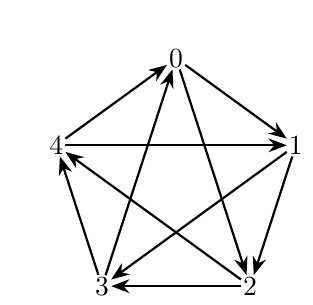
\begin{tikzpicture}[
scale=0.8, 
    >=Stealth,
    node/.style={inner sep=0.6pt} % 去掉 circle, draw
]

% 五个点，按逆时针标号 0,1,2,3,4
\node[node] (0) at (90:2)   {0};   % 上
\node[node] (1) at (18:2)   {1};   % 右上
\node[node] (2) at (-54:2)  {2};   % 右下
\node[node] (3) at (-126:2) {3};   % 左下
\node[node] (4) at (162:2)  {4};   % 左上

% 0 指向 1, 2
\draw[->,line width=0.8pt] (0) -- (1);
\draw[->,line width=0.8pt] (0) -- (2);

% 1 指向 2, 3
\draw[->,line width=0.8pt] (1) -- (2);
\draw[->,line width=0.8pt] (1) -- (3);

% 2 指向 3, 4
\draw[->,line width=0.8pt] (2) -- (3);
\draw[->,line width=0.8pt] (2) -- (4);

% 3 指向 4, 0
\draw[->,line width=0.8pt] (3) -- (4);
\draw[->,line width=0.8pt] (3) -- (0);

% 4 指向 0, 1
\draw[->,line width=0.8pt] (4) -- (0);
\draw[->,line width=0.8pt] (4) -- (1);

\end{tikzpicture}
\caption{circulant digraph $G=\vec{C}_5^{1,2}$} 
\label{fig:C512} 
\end{figure}

We have the following simple observations:
\begin{itemize}
  \item $e_{012}\in\Omega_2(G)$, $e_{013}\notin\Omega_2(G)$, $e_{013}-e_{023}\in\Omega_2(G)$;
  \item $e_{0123}\in\Omega_3(G)$, $e_{0124}-e_{0134}+e_{0234}\in\Omega_3(G)$;
  \item $e_{01234}\in\Omega_4(G)$, $e_{02340}-e_{01340}+e_{01240}-e_{01230}\in\Omega_4(G)$;
  \item For each vertex $a\in\mathbb{Z}_5$, the following elementary path is $\partial$-invariant:
  $$e_{a,(a+1),(a+2),\ldots,(a+n)}\in\Omega_{n}(G),\qquad a+j\pmod 5.$$
\end{itemize}

Thus, the path complex $\Omega_*(G;\mathbb{K})$ is infinite dimensional, where for each $n\in\Z_{\geq0}$, $\Omega_n(G;\mathbb{K})\neq0$. More explicitly, we have the following result.

\begin{lemma}\label{basis} For the circulant digraph $G=\vec{C}_5^{1,2}$, we have
\[\dim_{\mathbb{K}}\Omega_n(G;\mathbb{K})=10,\quad \forall~n\geq1.\]
Each vertex $a\in\Z_5$ gives two generators:
\begin{align*}
\alpha_a^{(n)}=~&e_{a,(a+1),(a+2),\ldots,(a+n)},\\
\beta_a^{(n)}=~&\sum_{j=1}^n(-1)^{n-j}e_{a,a+1,\ldots,a+j-1,a+j+1,a+j+2,\ldots,a+n+1}.
\end{align*}
Here all the vertices are understood modulo $5$.
\end{lemma}



\begin{proof} (1) It is easy to check that 
\[\alpha_a^{(n)},\beta_a^{(n)}\in\Omega_n(G;\mathbb{K}).\]
And $\alpha_a^{(n)}$ is the unique chain containing the elementary path $e_{a,a+1,\dots,a+n}$, and $\beta_a^{(n)}$ is the unique chain containing the elementary path $e_{a,a+2,a+3,\dots,a+n+1}$. Thus, all of the ten paths are linearly independent. Then we have $\dim_{\mathbb{K}}\Omega_n(G;\mathbb{K})\geq10$. 

On the other hand, for each vertex $a\in\Z_5$, let $A_n(a)\subset A_n$ be the span of allowed $n$-paths starting at $a$.
Then $A_n=\bigoplus_{a\in\Z_5} A_n(a)$ and $\Omega_n=\bigoplus_{a\in\Z_5} \Omega_n(a)$ where
\[\Omega_n(a):=\Omega_n\cap A_n(a).\]
It follows from the following lemma \ref{lem:fixed-start-2dof} that $\dim \Omega_n(a)\le 2$  .

Thus, $\dim_{\mathbb{K}}\Omega_n(G;\mathbb{K})\leq10$, $n\geq1$. Then $\left\{\alpha_a^{(n)},\beta_a^{(n)}\right\}_{a\in\Z_5}$ is a basis of $\Omega_{n}(G;\mathbb{K})$.
\end{proof}



\begin{lemma}
\label{lem:fixed-start-2dof}
Fix $n\ge 2$ and $a\in\Z_5$.
Encode an allowed $n$-path starting at $a$ by its step word
\[w=(\varepsilon_1,\dots,\varepsilon_n)\in\{1,2\}^n,\]
which means that the path is
\[e_w=e_{a, a+\varepsilon_1, a+\varepsilon_1+\varepsilon_2, \cdots,~ a+\varepsilon_1+\cdots+\varepsilon_n}\quad(\mathrm{mod}\ 5).\]
Write any chain in $A_n(a)$ as $P=\sum_w c_w\,e_w$.
Then the condition $P\in\Omega_n(a)$ forces:
\begin{enumerate}
\item If $w$ contains the substring $22$ anywhere, then $c_w=0$.
\item For each position $j\in\{1,\dots,n-1\}$ and for each fixed context (letters outside positions $j,j+1$),
if $w=\cdots 12\cdots$ and $w'=\cdots 21\cdots$ differ only by swapping $12\leftrightarrow 21$ at $j,j+1$, then
\[c_w+c_{w'}=0.\]
\end{enumerate}
Consequently, $c_w=0$ for every word containing at least two occurrences of $2$.
Moreover, among words containing exactly one $2$, the coefficients are determined up to a single scalar by the sign rule
obtained from repeated swaps.
Therefore $\dim\Omega_n(a)\le 2$.
\end{lemma}


\begin{proof}
By definition of the boundary operator $\partial$, 
if the consecutive steps are $(\varepsilon_j,\varepsilon_{j+1})$, then the merged step is
$\varepsilon_j+\varepsilon_{j+1}\in\{2,3,4\}$.
In this circulant digraph $G$, only steps $1$ and $2$ are edges, so a merged step $3$ or $4$ produces a forbidden face.
The definition $x\in\Omega_n(a)$ is equivalent to requiring that every forbidden face has coefficient $0$ in $\partial x$.
We now read off the resulting linear equations.

\smallskip
\noindent\textbf{(i) Words containing $22$ vanish.}
Suppose $w$ contains $22$ at positions $j,j+1$.
Deleting the interior vertex between these two steps produces a face with a merged step $4$ at that location.
No other allowed word produces the same face with a step $4$ at the same location (because the only way to get $4$ is $2+2$).
Hence the coefficient of that forbidden face in $\partial x$ is exactly $\pm c_w$.
Requiring it to be $0$ forces $c_w=0$.

\smallskip
\noindent\textbf{(ii) Swapping $12$ and $21$ flips sign.}
Fix $j\in\{1,\dots,n-1\}$ and fix all letters of the word outside positions $j,j+1$.
There are exactly two allowed local patterns whose sum is $3$, namely $12$ and $21$.
Deleting the interior vertex between these two steps produces the same forbidden face with merged step $3$.
Moreover, in \eqref{eq:boundary} the sign $(-1)^j$ attached to deleting that vertex is the same for both words.
Therefore the coefficient of this forbidden face in $\partial x$ is $\pm(c_w+c_{w'})$, and requiring it to vanish gives
$c_w+c_{w'}=0$.

\smallskip
\noindent\textbf{(iii) Eliminating words with two or more $2$'s.}
Let $w$ contain at least two $2$'s.
If it contains $22$, then $c_w=0$ by (i).
Otherwise, between any two $2$'s there is at least one $1$.
Using (ii), we may swap an adjacent $21$ to $12$ (picking up a sign) and thereby move a $2$ one position to the right.
Repeating, we can move a $2$ across a string of $1$'s until it becomes adjacent to the next $2$, producing a word that contains $22$.
The coefficient of that adjacent word is $\pm c_w$ after the sequence of swaps.
By (i) it must be $0$, hence $c_w=0$.

\smallskip

In summary, the only potentially nonzero coefficients are:
\begin{itemize}
    \item[(a)] the all-$1$ word $1\cdots 1$ (one scalar), and
    \item[(b)] words with exactly one $2$. Any two such words differ by moving the unique $2$ through adjacent swaps; by (ii) each swap flips the sign, so all these coefficients
are determined by a single scalar.
\end{itemize}
Thus $\Omega_n(a)$ is spanned by two elements, hence $\dim\Omega_n(a)\le 2$.
\end{proof}


\begin{theorem}\label{thm1} The path homologies of the circulant digraph $G$ are given by
\[H_n^{\mathrm{path}}(G;\mathbb{K})\cong\begin{cases}
\mathbb{K} &\quad n=0,1\\
0 &\quad n\geq2
\end{cases}~.\]
\end{theorem}

\begin{proof}

 Let $s_n:=(-1)^n$. Using the basis in Lemma \ref{basis}, we have the following explicit formulas
(for $n\ge 3$, and again all indices mod $5$):
\begin{equation}\label{eqrec}
\begin{aligned}
 \partial \alpha_a^{(n)}&=s_n\alpha_a^{(n-1)}+\beta_{a+1}^{(n-1)}- s_n\beta_a^{(n-1)},\\
 \partial \beta_a^{(n)}&=s_n\alpha_a^{(n-1)}-s_n\alpha_{a+2}^{(n-1)}- s_n\beta_a^{(n-1)}+\beta_{a+1}^{(n-1)}.
\end{aligned}
\end{equation}
\vskip 0.2cm

Consider the digraph map (rotation or shift automorphism)
$$\tau:G\rightarrow G,\quad \tau(a)=a+1\pmod5.$$
Immediately we have
\begin{itemize}
\setlength\itemsep{0pt}
\item $\tau$ is an isomoprhism of $G$;
\item $\Omega_n(G;\mathbb{K})$ is $\tau$-invariant; in particular,
\[\tau\alpha_a^{(n)}=\alpha_{a+1}^{(n)},\qquad \tau\beta_a^{(n)}=\beta_{a+1}^{(n)}.\]
\item The boundary operator $\partial$ commutes with $\tau$.
\end{itemize}

Then we can compute the rank of $\partial_n$ by decomposing into $\tau$-eigenspaces. Over a field containing a primitive fifth root of unity (e.g. over $\mathbb{C}$), $\tau$ is diagonalizable with eigenvalues $\lambda$ satisfying $\lambda^5=1$. 


For such a $\lambda$, define the Fourier modes
\[
\alpha^{(n)}_\lambda:=\sum_{a\in\Z_5}\lambda^{-a}\,\alpha^{(n)}_a,\qquad
\beta^{(n)}_\lambda:=\sum_{a\in\Z_5}\lambda^{-a}\,\beta^{(n)}_a.
\]
A change of variables $b=a+1$ shows
\[
\tau \alpha^{(n)}_\lambda=\sum_a \lambda^{-a}\alpha^{(n)}_{a+1}
=\sum_b \lambda^{-(b-1)}\alpha^{(n)}_b
=\lambda\sum_b \lambda^{-b}\alpha^{(n)}_b
=\lambda \alpha^{(n)}_\lambda,
\]
and similarly $\tau \beta^{(n)}_\lambda=\lambda \beta^{(n)}_\lambda$.  Since the $\lambda$-eigenspace inside $\Omega_n$ has
dimension $2$ (one $\alpha$-type and one $\beta$-type generator), the pair $(\alpha^{(n)}_\lambda,\beta^{(n)}_\lambda)$ spans the $\lambda$-eigenspace.

Now applying the explicit boundary recursions \eqref{eqrec}, we can compute
\begin{align*}
\partial_n \alpha^{(n)}_\lambda
&=\sum_a \lambda^{-a}\partial_n \alpha^{(n)}_a\\
&=\sum_a \lambda^{-a}\Bigl(s_n\alpha^{(n-1)}_a+\alpha^{(n-1)}_{a+1}-s_n\beta^{(n-1)}_a\Bigr)\\
&=s_n\alpha^{(n-1)}_\lambda+\sum_a \lambda^{-a}\alpha^{(n-1)}_{a+1}-s_n\beta^{(n-1)}_\lambda\\
&=s_n\alpha^{(n-1)}_\lambda+\lambda \alpha^{(n-1)}_\lambda-s_n\beta^{(n-1)}_\lambda\\
&=(s_n+\lambda)\alpha^{(n-1)}_\lambda+(-s_n)\beta^{(n-1)}_\lambda.
\end{align*}
Similarly, we have
\begin{align*}
\partial_n \beta^{(n)}_\lambda
&=\sum_a \lambda^{-a}\partial_n \beta^{(n)}_a\\
&=\sum_a \lambda^{-a}\Bigl(s_n\alpha^{(n-1)}_a-s_n\alpha^{(n-1)}_{a+2}-s_n\beta^{(n-1)}_a+\beta^{(n-1)}_{a+1}\Bigr)\\
&=s_n\alpha^{(n-1)}_\lambda-s_n\sum_a \lambda^{-a}\alpha^{(n-1)}_{a+2}-s_n\beta^{(n-1)}_\lambda+\sum_a \lambda^{-a}\beta^{(n-1)}_{a+1}\\
&=s_n\alpha^{(n-1)}_\lambda-s_n\lambda^2\alpha^{(n-1)}_\lambda-s_n\beta^{(n-1)}_\lambda+\lambda\beta^{(n-1)}_\lambda\\
&=s_n(1-\lambda^2)\alpha^{(n-1)}_\lambda+(\lambda-s_n)\beta^{(n-1)}_\lambda.
\end{align*}
Thus, with respect to the eigenbases $(\alpha^{(n)}_\lambda,\beta^{(n)}_\lambda)$ and $(\alpha^{(n-1)}_\lambda,\beta^{(n-1)}_\lambda)$, the matrix of $\partial_n$ is given by
\[M_{s_n}(\lambda)=\begin{pmatrix}
s_n+\lambda & -s_n\\
s_n(1-\lambda^2) & \lambda-s_n.
\end{pmatrix}\]

A direct determinant computation gives (using $s_n=(-1)^n$)
\[\det M_{s_n}(\lambda)=(s_n+\lambda)(\lambda-s_n)-(-s_n)\cdot s_n(1-\lambda^2)=(\lambda^2-1)+(1-\lambda^2)=0.\]
Thus each block has rank at most 1. The entry $-s_n\neq0$, thus $M_{s_n}(\lambda)$ is a rank one 2-by-2 matrix. Since there are five eigenvalues, the total rank is $5$. Thus, for $n\geq3$, we have
\begin{align*}
 &\dim\im(\partial_n)=\rank(\partial_n)=5,\\
 &\dim\ker(\partial_n)=\dim\Omega_n-\rank{\partial_n}=10-5=5.
\end{align*}
Thus $H_n^{\mathrm{path}}(G;\K)=0$, for $n\geq3$. It is easy to compute that 
\[H_2^{\mathrm{path}}(G;\K)=0,\quad H_1^{\mathrm{path}}(G;\K)=\K[e_{01}+e_{12}+e_{23}+e_{34}+e_{40}],\quad H_0^{\mathrm{path}}(G;\K)\cong\K.\]
\end{proof}


\begin{remark}
For simplicity, we introduce the stronger condition in our paper \cite{TY1,TY2}, and define the resulting path complex $H^{\sr}(G;\K)$ and cellular complex $H^{\cell}(G;\K)$ of the digraph $G$. In particular, we compute the two homologies (Example 4.3 in \cite{TY2}) of this example, we also get
\[
H_n^{\sr}(G;\K)\cong H_n^{\cell}(G;\K)\cong H_n^{\mathrm{path}}(G;\K)\cong
\begin{cases}
    \K & n=0,1\\
    0 & n\geq2
\end{cases}~.
\]
\end{remark}





\bigskip
\section{Circulant digraphs and the path complex}
In this section, we systematically study the path complex of circulant digraphs and compute the path homology in some special cases.
\subsection{Circulant digraphs}\label{sub:circulant}

\begin{definition}[Cayley digraph]
Let $H$ be a (finite) group and $S\subset H$ with the unit $1\notin S$. The \emph{Cayley digraph} $G=\Cay(H,S)$ has vertex set $V=H$ and a directed edge $a\rightarrow as$ for each $a\in H$, $s\in S$.    
\end{definition}

\begin{remark}
If $S=S^{-1}$, we usually regard $G$ as an undirected $|S|$-regular Cayley graph.
\end{remark}

\begin{proposition}
There are many basic properties for the Cayley digraphs:
\begin{itemize}
    \item \textbf{vertex transitivity:} Left mulitiplication $L_h:a\mapsto ha$ is an automorphism of $\Cay(H,S)$ for every $h\in H$. In particular, Cayley digraphs are vertex-transitive.
    \item \textbf{connectivity:} $\Cay(H,S)$ is (strongly) connected if and only if $\langle S\rangle=H$.
\end{itemize}
\end{proposition}


Fix an integer $n\geq 3$.  Let $\mathbb Z_n=\mathbb Z/n\mathbb Z$ and let $S\subset\Z_n$ be a subset, $0\notin S$.

The \emph{circulant directed graph} $\vec{C}_n^S$ is the Cayley digraph 
$\Cay(\Z_n,S)$. That is, it has vertex set $V=\mathbb Z_n$ and an arrow
\[
a\longrightarrow a+s\quad\text{for each }a\in\mathbb Z_n,\ s\in S.
\]
This is the Cayley digraph of the cyclic group $\mathbb Z_n$ with connection set $S$. The example in the previous section is exactly $\vec{C}_5^{1,2}$. The circulant digraphs are important from several viewpoints: symmetry and classification, spectral/Fourier analysis, extremal and structural graph theory, algorithmic routing and fault-tolerance, network design, and interactions with topology (path homology) and operator algebras (graph $C^\ast$-algebras). 

\begin{remark}
One can also realize the circulant digraph from the matrix viewpoint. That is, the adjacency matrix of $\vec{C}_n^S$ is a circulant matrix. For $\vec{C}_5^{1,2}$, its adjacency matrix is given by
\[A=\begin{pmatrix}
    0 & 1 & 1 & 0 & 0\\
    0 & 0 & 1 & 1 & 0\\
    0 & 0 & 0 & 1 & 1\\
    1 & 0 & 0 & 0 & 1\\
    1 & 1 & 0 & 0 & 0
\end{pmatrix}.\]
Such a circulant matrix is diagonal by the discrete Fourier transform. This is the engine behind explicit spectral formulas and fast algorithms. 
\end{remark}

Now let us focus on the structure of path complex of the circulant digraph $G=\vec{C}_n^S$. 

First, we write the elementary $m$-path $e_{v_0,v_1\ldots,v_m}$ as
\begin{equation}\label{elementarypath2}
(v_0;~s_1,\ldots,s_m),\qquad s_j=v_j-v_{j-1},~~~j=1,2\ldots,m.
\end{equation}
It is an allowed elementary $m$-path if and only if all $s_j\in S$.

Let $p_m$ be the elementary $m$-path in $G$. 
Then
\[A_m(G)=\Span_{\K}\{p_m\}\cong \K[\Z_n]\otimes (\K^S)^{\otimes m}.\]

If $j$ is a starting or ending vertex of an allowed elementary path, the face is automatically allowed.
If $1\le j\le n-1$ is internal, deleting $v_j$ merges two consecutive steps:
\[
(s_j,s_{j+1}) \mapsto s_j+s_{j+1} \pmod n.
\]
Hence an internal face is allowed if and only if $s_j+s_{j+1}\in S$ (mod $n$).



\subsection{Low-dimensional path chains \texorpdfstring{$\Omega_2$, $\Omega_3$}{Omega2, Omega3} in circulant digraphs}\label{sub:lowdim}

Define a set
\[F:=(S+S)\setminus S \pmod n.\]
And we call $F$ the set of illegal merged steps. For $r\in\Z_n$, define the decomposition number
\[N(r):=\#\{(s,t)\in S\times S:\ s+t\equiv r\pmod n\}.\]

\subsubsection{\texorpdfstring{$\Omega_2(\vec{C}_n^S)$}{Omega2}}
\begin{proposition}[Linear constraints for $\Omega_2$]\label{prop:Omega2}
Fix a starting vertex $a\in\Z_n$.  An allowed $2$-path
$$
u=\sum_{s,t\in S} c_{s,t}\,e_{a,a+s,a+s+t}\in \Omega_2
$$
if and only if for every illegal $r\in F$, we have
\[
\sum_{s+t=r} c_{s,t}=0.
\]
Equivalently, for each illegal $r\in F$, the coefficients on the $N(r)$ paths with merged step $r$
have total sum $0$, hence contribute a subspace of dimension $N(r)-1$ (if $N(r)\ge 1$).
\end{proposition}

\begin{proof} The proof follows from definition.
\end{proof}


\begin{definition}\label{def:Wcycle}
For $|S|\geq2$, $\{s,t\}\subset S$ and $a\in\mathbb Z_n$, we define the commutator square as follows
\[
\operatorname{comm}_a(s,t):=e_{a,a+s,a+s+t}\;-\;e_{a,a+t,a+s+t}.\footnote{For $|S|=1$, this commutator square is automatically 0.}
\]
Let its translation-average be
\[
W^{s,t}:=\sum_{a\in\mathbb Z_n}\operatorname{comm}_a(s,t)\in A_2(\vec{C}_n^S).
\]
\end{definition}

\begin{lemma}\label{lem:Wcycle}
For $|S|\ge 2$ and any distinct $s,t\in S$, we have 
\[W^{s,t}=-W^{t,s}\in\Omega_2(\vec{C}_n^S)\quad\text{ and }\quad \partial W^{s,t}=0.\]
\end{lemma}

\begin{proof}
The middle-deletion faces in $\partial(\operatorname{comm}_a(s,t))$ cancel, so each
$\operatorname{comm}_a(s,t)$ lies in $\Omega_2(\vec{C}_n^S)$.  A direct expansion gives
\[
\partial(\operatorname{comm}_a(s,t))
=e_{a,a+s}-e_{a,a+t}+e_{a+s,a+s+t}-e_{a+t,a+s+t}.
\]
Summing over $a$ yields telescopic cancellation in pairs, hence $\partial W^{s,t}=0$.
\end{proof}

Whether $W^{s,t}$ survives in $H_2^{\mathrm{path}}(\vec{C}_n^S)$ depends on whether the graph has enough ``diagonals'' to fill it by $3$-chains.

\subsubsection{\texorpdfstring{$\Omega_3(\vec{C}_n^S)$}{Omega3}}

\begin{proposition}\label{prop:P}
Assume $|S|\geq2$ and  $s,t,r\in S$ satisfy $r\equiv s+t\pmod n$. Define the translation-average $3$-chain
\[
P^{s,t}:=\sum_{a\in\mathbb Z_n}e_{a,a+s,a+r,a+r+s}.
\]
Then $P^{s,t}\in \Omega_3(\vec{C}_n^S)$ and
\[
\partial P^{s,t}= W^{s,r}-W^{s,t}.
\]
Consequently, $[W^{s,r}]=[W^{s,t}]$ in $H_2^{\mathrm{path}}(\vec{C}_n^S)$.  
\end{proposition}

\begin{proof}
It is easy to compute
\begin{align*}
\partial e_{a,a+s,a+r,a+r+s}=~&e_{a+s,a+r,a+r+s}-e_{a,a+r,a+r+s}+e_{a,a+s,a+r+s}-e_{a,a+s,a+r}\\
=~&e_{a+s,a+r,a+r+s}-e_{a,a+s,a+r}+\operatorname{comm}_a(s,r)\\
=~&(a+s;~t,s)-(a;~s,t)+\operatorname{comm}_a(s,r)\quad (\text{by notation} \eqref{elementarypath2})
\end{align*}
Thus, summing over $a\in\Z_n$, we arrive at
\[\partial P^{s,t}= W^{s,r}-W^{s,t}.\]
\end{proof}


\begin{remark}
This proposition is the precise GLMY analogue of the geometric statement:
a diagonal edge $r=s+t$ triangulates a square and kills its fundamental $2$-cycle.
This explains, for example, why $S=\{1,2\}$ has $H_2^{\mathrm{path}}(\vec{C}_5^{1,2})=0$ (the diagonal $1+1=2$ is present),
while $S=\{1,s\}$ with $s\neq 2$ often has a surviving $2$-class.
\end{remark}



We have seen that the low-dimensional path complex is controlled by how many additive relations $s+t\in S$ exist. We will understand the additive property of $S$ in terms of another two examples in the appendix \ref{appendix}.


 


\subsection{Special cases}\label{sub:special}

\subsubsection{The case \texorpdfstring{$S=\{1\}$}{S1}}

In this case, we have $\langle S\rangle=\Z_n$. Thus, the digraph $\vec{C}_n^1$ is strongly connected. In particular, it is easy to obtain
\begin{itemize}
    \item[(1)] For $n=2$, the corresponding digraph is contractible, then 
    \[H_m(\vec{C}_2^1;\K)=\begin{cases}
        \K & m=0\\
        0 & m\ge 1.
    \end{cases}\] 
    \item[(2)] For $n>2$, the corresponding digraph is given by a monotone cycle. Then
    \[H_m(\vec{C}_n^1;\K)=\begin{cases}
        \K & m=0,1\\
        0 & m\ge 2.
    \end{cases}\]
\end{itemize}


\subsubsection{The case \texorpdfstring{$n\ge 5$, $S=\{1,s\}$, $1<s<n/2$}{S1s}.}
In this case, consider an allowed elementary $2$-path $e_{a,a+l,a+l+m}$ with $l,m\in\{1,s\}$.
The internal face deletion merges $l+m$.
Since $1<s<n/2$, the sums $2$, $s+1$ and $2s$ are distinct integers in $\{2,\dots,n-1\}$.

\begin{lemma} For $n\ge 5$, $S=\{1,s\}$, $1<s<n/2$, we have the following complete description for $\Omega_*(\vec{C}_n^S)$.
\begin{itemize}
\item[(1)] If $s=2$, then for $m\ge1$, $\Omega_m$ has a $2n$-element basis $\{\alpha_a^{(m)},\beta_a^{(m)}\}_{a\in\Z_n}$, where
\begin{align*}
\alpha_a^{(m)}=~&e_{a,(a+1),(a+2),\ldots,(a+m)},\\
\beta_a^{(m)}=~&\sum_{j=1}^m(-1)^{m-j}e_{a,a+1,\ldots,a+j-1,a+j+1,a+j+2,\ldots,a+m+1}.
\end{align*}
\item[(2)] If $s\ne 2$, then $\Omega_2$ has an $n$-element basis $\{\gamma_a\}_{a\in\Z_n}$, where
\[
 \gamma_a=e_{a,a+1,a+1+s}-e_{a,a+s,a+1+s}=\operatorname{comm}_a(1,s),
\]
and $\Omega_m(\vec{C}_n^S)=0$, $m\geq3$.
\end{itemize}
\end{lemma}

\begin{proof}
(1) The proof for the case $S=\{1,2\}$ is the same as the one of Lemma \ref{basis}. 

\vskip 0.2cm
(2) We write the allowed elementary $2$-path $e_{a,a+s_1,a+s_1+s_2}$ as $(a;~s_1,s_2)$, and call it the pattern $(s_1,s_2)$. For $s\neq2$, 
\begin{itemize}
    \item the boundary of the pattern $(1,1)$ produces illegal path $e_{a,a+2}$;
    \item the boundary of the pattern $(s,s)$ produces illegal path $e_{a,a+2s}$;
    \item the mixed patterns $(1,a)$ and $(a,1)$ both produce the same illegal path $e_{a,a+s+1}$, but the difference $\gamma_a$ cancels it, so $\gamma_a\in\Omega_2(\vec{C}_n^S)$.
\end{itemize}
For $m\geq3$, again we write an allowed elementary $m$-path as
\[(a;~s_1,s_2,\ldots,s_m),\quad s_i\in\{1,s\}.\]
Similarly, we have the following result.
\begin{itemize}
    \item If $(s_j,s_{j+1})=(1,1)$ for some $1\le j\le m-1$, then the internal face obtained by deleting the $j$-th vertex
has, at position $j$, a merged increment $2$.
Moreover this illegal $(m-1)$-face cannot arise as an internal face of any other allowed elementary $m$-path.
\item If $(s_j,s_{j+1})=(s,s)$ for some $1\le j\le n-1$, then the analogous statement holds with merged increment $2s$.
\end{itemize}
Assume $P\in\Omega_m(\vec{C}_n^S)$, $m\ge3$, then every elementary appearing in $P$ is forced to be of the form
\[(a;~1,s,1,s,\ldots)\quad\text{or}\quad (a;~s,1,s,1,\ldots).\]
Now let us investigate the $j=1$ internal deletion face. 
\begin{itemize}
    \item For elementary path $(a;~1,s,1,s,\ldots)$, deleting the first internal vertex merges $(1,s)$ into the illegal path $(a;~s+1,1,s,\ldots)$.
    \item For elementary path $(a;~s,1,s,1,\ldots)$, deleting the first internal vertex merges $(s,1)$ into the illegal path $(a;~s+1,s,1,\ldots)$.
\end{itemize}
The resulting illegal faces are distinct. Thus, their coefficients in $\partial P$ must vanish, forcing the coefficients of both kinds of elementary path in $P$ to be zero. Hence $P=0$, which means that 
\[\Omega_m(\vec{C}_n^S)=0, \quad m\geq3.\]
\end{proof}


\begin{theorem}\label{thm:1s}
For the circulant digraph $\vec{C}_n^S$ with $n\ge5$, $S=\{1,s\}$, $1<s<n/2$. 
\begin{itemize}
    \item[(1)] If $s=2$, then
    \[H_0^{\mathrm{path}}\cong\K,\quad H_1^{\mathrm{path}}\cong\K,\quad H_m^{\mathrm{path}}\cong0,~m\geq2.\]
    \item[(2)] If $s\neq2$, then
    \[H_0^{\mathrm{path}}\cong\K,\quad H_1^{\mathrm{path}}\cong\K^2,\quad H_2^{\mathrm{path}}\cong\K,\quad H_m^{\mathrm{path}}\cong0,~m\geq3.\]
\end{itemize}
\end{theorem}

\begin{proof}
(1) It is similar to the proof of Theorem \ref{thm1}. Using the Fourier modes, one can reduce the rank computation to the $\tau$-eigenspaces. Then we have
\[\rank(\partial_1)=n-1,\qquad \rank(\partial_m)=n,~~ m\geq2.\]
It follows that 
\[\dim H_1^{\mathrm{path}}=(2n-(n-1))-n=1,\quad H_{m\geq2}^{\mathrm{path}}=0.\]

(2) For $s\neq2$, the path complex of $\vec{C}_n^{S}$ is just
\[0~\rightarrow~\Omega_2~\xrightarrow{\partial_2}~\Omega_1~\xrightarrow{\partial_1}~\Omega_0~\rightarrow ~0.\]
A Fourier diagonalization (or an explicit circulant matrix computation, see more details in the next section) gives $\rank(\partial_2)=n-1$.
Hence 
\[\dim H_2^{\mathrm{path}}=1,\qquad \dim H_1^{\mathrm{path}}=(2n-(n-1))-(n-1)=2.\]
\end{proof}



\subsubsection{The case \texorpdfstring{$S=\{1,2,\ldots,d\}$, $2<d<n/2$}{S12d}} 


For $S=\{1,2,\ldots,d\}$, $2<d<n/2$, the natural digraph embedding $\vec{C}_n^{1,2}\hookrightarrow \vec{C}_n^S$ induces that chain map
\[i:\ \left(\Omega_*(\vec{C}_n^{1,2}),\partial\right)\ \to\ \left(\Omega_*(\vec{C}_n^S),\partial\right).\]
What is more important, $i$ has a homotopy inverse.

\begin{theorem}\label{thm:S12d} 
For $S=\{1,2,\ldots,d\}$, $2<d<n/2$. Let $i$ be the above chain map.
Then there exists a chain map
\[
\Pi:\ \left(\Omega_*(\vec{C}_n^S),\partial\right)~\rightarrow~ \left(\Omega_*(\vec{C}_n^{1,2}),\partial\right)
\]
such that $\Pi\circ i=\mathrm{Id}_{\Omega_*(\vec{C}_n^{1,2})}$ and $i\circ\Pi$ is chain-homotopic to $\mathrm{Id}_{\Omega_*(\vec{C}_n^S)}$.
\end{theorem}

\begin{proof} 
First we write an allowed elementary $m$-path in $\vec{C}_n^S$ as
\[
p=e_{v_0v_1\cdots v_m}\equiv (v_0;~ s_1,\dots,s_m),
\qquad s_r:=v_r-v_{r-1}\in\{1,\dots,d\}.
\]

\medskip
Define the \emph{long-step defect} of $p$ by
\[
E(p):=(e_1,\dots,e_m),\qquad e_r:=\max\{0,s_r-2\}\in\{0,1,\dots,d-2\}.
\]
Thus $E(p)=(0,\dots,0)$ iff every step has length $1$ or $2$, i.e.\ $p$ is an allowed $m$-path in $\vec{C}_n^{1,2}$.

We order defect profiles lexicographically:
\[
E(p)<_{\mathrm{lex}}E(q)\quad\Longleftrightarrow\quad
\exists\,r\ \text{s.t. } e_1=\cdots=e_{r-1}=e'_1=\cdots=e'_{r-1}\ \text{and } e_r<e'_r.
\]
For a finite chain $u=\sum c_p\,p\in\Omega_m(\vec{C}_n^S)$, we write
\[
E_{\max}(u):=\max\nolimits_{<_{\mathrm{lex}}}\{\,E(p): c_p\neq 0\,\}.
\]
This is a well-defined element of $\{0,\dots,d-2\}^m$.

\medskip
\noindent\textbf{Step 1: the homotopy operator $h$ and the restriction lemma.}
Define $h$ on elementary allowed $m$-paths $p=(v_0;~s_1,\dots,s_m)$ as follows.
If $E(p)=(0,\dots,0)$, set $h(p)=0$.  Otherwise, let
\[
j=j(p):=\min\{\,r\in\{1,\dots,m\}:\ s_r\ge 3\,\}.
\]
Write $s_j=\ell\ge 3$ and set
\[
h(p):=(-1)^{j+1}\,(v_0;\ s_1,\dots,s_{j-1},\,1,\,\ell-1,\,s_{j+1},\dots,s_m)\in A_{m+1}(\vec{C}_n^S).
\]
Equivalently, in vertex notation, we insert the intermediate vertex $v_{j-1}+1$ between $v_{j-1}$ and $v_j$.
Since $S=\{1,\dots,d\}$ and $\ell-1\in\{2,\dots,d-1\}$, $h(p)$ is still allowed.

Extend $h$ $\K$-linearly to $A_*(\vec{C}_n^S)$, and define
\[
\pi:=\mathrm{Id}-(\partial h+h\partial).
\]
On the full regular path space $\Lambda_*(\Z_n;\K)$ one has $\partial^2=0$, hence $\pi$ is a chain map:
$\partial\pi=\pi\partial$.

\begin{lemma}[Restriction lemma]
For every $m\ge 0$, $\pi$ preserves the GLMY subspaces:
\[
\pi\bigl(\Omega_m(\vec{C}_n^S)\bigr)\subset \Omega_m(\vec{C}_n^S).
\]
In particular, $\pi$ is a chain map on $(\Omega_*(\vec{C}_n^S),\partial)$ and $\pi|_{\Omega_*(\vec{C}_n^{1,2})}=\mathrm{Id}$.
\end{lemma}

\begin{proof}
Take $u\in\Omega_m(\vec{C}_n^S)$.  By definition, $u\in A_m(\vec{C}_n^S)$ and $\partial u\in \Omega_{m-1}(\vec{C}_n^S)\subset A_{m-1}(\vec{C}_n^S)$.
We must show $\pi(u)\in A_m(\vec{C}_n^S)$ (allowedness) and then $\partial(\pi(u))\in \Omega_{m-1}$ follows from
$\partial\pi=\pi\partial$.

\medskip\noindent
\textbf{(i) Allowedness of $h\partial u$.}
Since $\partial u\in A_{m-1}$ and $h$ sends allowed elementary paths to allowed ones (it only inserts an intermediate
vertex along a step in $S$), we have $h(\partial u)\in A_m$.

\medskip\noindent
\textbf{(ii) Allowedness of $\partial h(u)$.}
Write $u=\sum c_p p$ as a linear combination of allowed elementary $m$-paths $p$.  Then
\[
\partial h(u)=\sum c_p\,\partial h(p).
\]
We claim that every non-allowed elementary $m$-path $q$ has zero coefficient in $\partial h(u)$.

Fix such a non-allowed $q$.  Since $h(p)$ is allowed, $q$ can only appear in $\partial h(p)$ as an interior face of $h(p)$, i.e.\ by deleting an interior vertex of $h(p)$ and merging two consecutive steps whose sum exceeds $d$.
Let $j=j(p)$ be the split index for $p$, and let the inserted vertex in $h(p)$ sit between the steps
$s_{j}$ (split into $1$ and $s_j-1$).
There are three types of interior deletions in $h(p)$:

\smallskip
\emph{Type 1: deletions away from the inserted vertex.}
If we delete an interior vertex not adjacent to the inserted one, the two merged increments in $h(p)$
are identical to a pair of adjacent increments in $p$ (with the same surrounding context).
Therefore the resulting merged increment in $q$ (which is $>d$) corresponds to a forbidden $(m-1)$-face of $p$
appearing in $\partial p$.

\smallskip
\emph{Type 2: delete the vertex immediately left of the inserted vertex.}
This merges $(s_{j-1},1)$ into $s_{j-1}+1$.  If this is $>d$, then necessarily $s_{j-1}=d$, and deleting the
corresponding vertex in $p$ merges $(s_{j-1},s_j)$ into $d+s_j>d$, hence again produces a forbidden face in $\partial p$.

\smallskip
\emph{Type 3: delete the vertex immediately right of the inserted vertex.}
This merges $(s_j-1,s_{j+1})$ into $(s_j-1)+s_{j+1}$.  If this exceeds $d$, then $s_j+s_{j+1}>d+1>d$, so deleting
the corresponding vertex in $p$ merges $(s_j,s_{j+1})$ into $s_j+s_{j+1}$, again a forbidden face in $\partial p$.

\medskip
In all cases, a forbidden $m$-face $q$ of $h(p)$ canonically determines a forbidden $(m-1)$-face $F(q)$ of $p$,
obtained by also deleting the inserted vertex (i.e.\ collapsing the split) after the interior deletion.
Moreover, for fixed $q$ the set of $p$ for which $q$ occurs in $\partial h(p)$ is exactly the set of $p$ for which
$F(q)$ occurs in $\partial p$ with the same outside context; the only difference is a global sign depending on the
relative position of the inserted vertex.  Concretely, one checks in the three cases above that the coefficient
contributed by a given $p$ satisfies
\[
\mathrm{coeff}_q(\partial h(p))=\pm\,\mathrm{coeff}_{F(q)}(\partial p),
\]
where the sign $\pm$ depends only on the deletion type (hence on $q$), not on $p$.

Therefore,
\[
\mathrm{coeff}_q(\partial h(u))
=\sum_{p} c_p\,\mathrm{coeff}_q(\partial h(p))
=\pm\sum_{p} c_p\,\mathrm{coeff}_{F(q)}(\partial p)
=\pm\,\mathrm{coeff}_{F(q)}(\partial u).
\]
But $u\in\Omega_m$ implies $\partial u\in A_{m-1}$, so every forbidden $(m-1)$-path has coefficient $0$ in $\partial u$.
In particular, $\mathrm{coeff}_{F(q)}(\partial u)=0$, hence $\mathrm{coeff}_q(\partial h(u))=0$.
This holds for every forbidden $q$, so $\partial h(u)\in A_m$.

\medskip
Combining (i) and (ii), we have
\[
\pi(u)=u-\partial h(u)-h\partial u\in A_m(\vec{C}_n^S).
\]
Similarly, $\partial u\in\Omega_{m-1}$, we also have
\[\partial(\pi(u))=\pi(\partial u)\in A_{m-1}.\] 
Hence $\pi(u)\in\Omega_m$.
The identity $\pi|_{\Omega_*(\vec{C}_n^{1,2})}=\mathrm{Id}$ follows from $h=0$ on defect-zero paths.
\end{proof}

\noindent\textbf{Step 2: chain-level decrease of the defect profile.}

\begin{lemma}[Lexicographic decrease on $\Omega_m$]
Let $m\ge 0$ and $u\in\Omega_m(\vec{C}_n^S)$.  If $E_{\max}(u)\neq (0,\dots,0)$, then
\[
E_{\max}\bigl(\pi(u)\bigr) <_{\mathrm{lex}} E_{\max}(u).
\]
Consequently, for every $u\in\Omega_m$ the sequence $u,\pi(u),\pi^2(u),\dots$ stabilizes after finitely many steps
to an element with defect profile $(0,\dots,0)$, i.e.\ supported on $\{1,2\}$-steps.
\end{lemma}

\begin{proof}
Write $u=\sum c_p p$ and let $E_{\max}(u)=E(p_0)$ for some $p_0$ in the support; choose $p_0$ so that
$E(p_0)$ is maximal and among those, the first long-step index $j(p_0)$ is minimal.

Consider $\pi(p_0)=p_0-(\partial h+h\partial)(p_0)$.  By construction, the face of $h(p_0)$ obtained by deleting the inserted
vertex is exactly $p_0$, and it appears in $\partial h(p_0)$ with coefficient $+1$ (this is why we chose the prefactor
$(-1)^{j+1}$).  Hence the term $p_0$ cancels in $\pi(p_0)$.

Now examine any elementary path $q$ that appears in $\pi(p_0)$ with nonzero coefficient and is allowed
(so $q$ can contribute to $E_{\max}(\pi(u))$).  Such a $q$ arises from:
\begin{enumerate}
\item an allowed face of $h(p_0)$ other than the one deleting the inserted vertex, or
\item an allowed term in $h(\partial p_0)$ (here we use that in $\Omega_m$ all forbidden faces cancel, so only allowed faces
      survive when we pass from $\partial p_0$ to $\partial u$ and then apply $h$).
\end{enumerate}
In either case, one checks directly on step-words that $q$ is obtained from $p_0$ by one of the following local moves:
\begin{itemize}
\item either the first long step $s_{j(p_0)}=\ell$ is replaced by $\ell-1$ (hence $e_{j(p_0)}$ decreases by $1$), or
\item the first long step is moved to the right (so the defect profile agrees up to a longer prefix of zeros/unchanged
      entries, hence becomes smaller in lex order once the split has propagated).
\end{itemize}
The only way to produce a term with the same defect profile as $p_0$ would be to create a new long step strictly
to the left of $j(p_0)$ by merging shorter steps inside $\partial p_0$ and then re-splitting via $h$.
But such contributions assemble into coefficients of forbidden faces in $\partial u$ (precisely the ``partial invariance''
issue noted in blue), and they vanish because $u\in\Omega_m$ implies $\partial u$ has no forbidden faces.
Therefore, among the allowed terms that survive in $\pi(u)$, none can have defect profile $\ge_{\mathrm{lex}}E(p_0)$,
and at least one strict decrease occurs because $p_0$ itself is cancelled.  This yields the claimed inequality
$E_{\max}(\pi(u))<_{\mathrm{lex}}E_{\max}(u)$.

Since the set of defect profiles $\{0,\dots,d-2\}^m$ is finite and $<_{\mathrm{lex}}$ is a well-order on it,
iterating $\pi$ must terminate at defect $(0,\dots,0)$.
\end{proof}

\textbf{Step 3: definition of $\Pi$ and the deformation retraction.}
For $u\in\Omega_m(\vec{C}_n^S)$, define $N(u)$ to be the number of strict decreases needed to reach defect $0$, i.e.
the smallest $N$ such that $E_{\max}(\pi^N(u))=(0,\dots,0)$. Define
\[
\Pi(u):=\pi^{N(u)}(u)\in \Omega_m(\vec{C}_n^{1,2}).
\]
Because $\pi$ is a chain map on $\Omega_*(\vec{C}_n^S)$ and $\Omega_*(\vec{C}_n^{1,2})$ is a subcomplex,
$\Pi$ is a chain map $\Omega_*(\vec{C}_n^S)\to \Omega_*(\vec{C}_n^{1,2})$.
Moreover, for $u\in\Omega_*(\vec{C}_n^{1,2})$ we have $h(u)=0$ hence $\pi(u)=u$ and thus $\Pi(u)=u$; therefore
$\Pi\circ i=\mathrm{Id}$.

\medskip
\noindent\textbf{Step 4: chain homotopy between $i\circ\Pi$ and $\mathrm{Id}$.}
Define, for $u\in\Omega_m(\vec{C}_n^S)$,
\[
H(u):=\sum_{k=0}^{N(u)-1} h\bigl(\pi^k(u)\bigr)\in \Omega_{m+1}(\vec{C}_n^S),
\]
where the sum is empty (hence $H(u)=0$) if $N(u)=0$.

Using $\pi=\mathrm{Id}-(\partial h+h\partial)$ and a telescoping sum,
\[
u-\pi^{N(u)}(u)=(\partial h+h\partial)\sum_{k=0}^{N(u)-1}\pi^k(u)=\partial H(u)+H(\partial u).
\]
Since $\Pi(u)=\pi^{N(u)}(u)$ and $i$ is inclusion, this identity reads
\[
\mathrm{Id}-i\circ \Pi=\partial H+H\partial,
\]
which exhibits $i\circ\Pi$ as chain-homotopic to the identity.  This completes the proof of Theorem~\ref{thm:S12d}.
\end{proof}


By homotopy invariance of path homology, we can reduce the  computation to digraph $\vec{C}_n^{1,2}$.
\begin{corollary} For $S=\{1,2,\ldots,d\}$, $2<d<n/2$, we have
\[H_0^{\mathrm{path}}(\vec{C}_n^{S})\cong \K,\qquad H_1^{\mathrm{path}}(\vec{C}_n^{S})\cong \K,\qquad H_m^{\mathrm{path}}(\vec{C}_n^{S})=0\ \ (m\ge 2).\]    
\end{corollary}


\bigskip

\section{Fourier block decomposition and no wrap-around \texorpdfstring{$S$}{S}}
\label{sec:Fourier}

Note that the circulant digraphs are among the simplest highly symmetric digraphs: the cyclic shift $\tau(a)=a+1$ is an automorphism of order $n$. This implies:
\begin{itemize}
\item \textbf{Vertex-transitivity}: all vertices look the same, so local computations globalize.
\item \textbf{Uniform degree}: $|S|$-out-arrows (and $|S|$-in-arrows).
\item \textbf{Group methods}: isomorphism, automorphisms, quotients, and lifts can be studied via group actions.
\end{itemize}

In this section, we will use the shift automorphism $\tau$ and Fourier ideas to study the path complex and path homology of circulant digraphs, as we have done for the example $\vec{C}_5^{1,2}$.
In particular, we will understand how $n$ and $S$ matter in the path homology in some sense.



\subsection{Fourier block decomposition}\label{sub:Fourier}

\begin{proposition}[Fourier block decomposition]\label{prop:Fourier}

Assume $\K$ contains all $n$-th roots of unity (e.g.\ $\K=\mathbb C$). For each $\lambda\in\K$ with $\lambda^n=1$, define the
$\lambda$-eigenspace
\[
\Omega_m^{(\lambda)}:=\{\,\alpha\in \Omega_m:\ \tau\alpha=\lambda\,\alpha\,\}.
\]
Then we have the direct sum decomposition
\begin{equation}\label{eq:fourier-split}
\Omega_m \cong \bigoplus_{\lambda^n=1} \Omega_m^{(\lambda)},\qquad
\partial(\Omega_m^{(\lambda)})\subset \Omega_{m-1}^{(\lambda)}.
\end{equation}
Each block is finite-dimensional, and the matrices of $\partial\big|_{\Omega_{*}^{(\lambda)}}$ have entries that are Laurent polynomials in $\lambda$. Consequently,
\begin{equation}\label{eq:homology-split}
H_m^{\mathrm{path}}(\vec{C}_n^S) \cong \bigoplus_{\lambda^n=1} H_m^{(\lambda)},\qquad
H_m^{(\lambda)}:=H_m(\Omega_*^{(\lambda)},\partial).
\end{equation}
\end{proposition}


\begin{proof} We have seen that for each $m\geq0$,
\[A_m(\vec{C}_n^S;\K)\cong \K[\Z_n]\otimes(\K^S)^{\otimes m}.\]
Then each $A_m(\vec{C}_n^S;\K)$ (thus $\Omega_m(\vec{C}_n^S)$) is finite dimensional. 

The automorphism $\tau:\vec{C}_n^S\rightarrow\vec{C}_n^S$ is of order $n$ and also induces an isomorphism
\[\tau:\left(\Omega_*(\vec{C}_n^S;\K),\partial\right)\rightarrow\left(\Omega_*(\vec{C}_n^S;\K),\partial\right).\]
Then the minimal polynomial $M(t)$ of $\tau$ divides $t^n-1$. Because $\K$ contains all $n$-th roots of unity and $\mathrm{char}(\K) = 0$, the polynomial $t^n-1$ splits into distinct linear factors, so $\tau$ is diagonalizable. Therefore,
\[\Omega_m(\vec{C}_n^S;\K) \cong \bigoplus_{\lambda^n=1} \Omega_m^{(\lambda)}(\vec{C}_n^S;\K),\qquad H_m^{\mathrm{path}}(\vec{C}_n^S) \cong \bigoplus_{\lambda^n=1} H_m(\Omega_*^{(\lambda)},\partial).\]

Let us write an allowed elementary $m$-path as $(a; ~s_1,\dots,s_m)$ with $s_i\in S$, and for each fixed word $w=(s_1,\dots,s_m)$, let $\{(a;w)\}_{a\in\Z_n}$ be its $\tau$-orbit. Passing to Fourier modes amounts to applying the discrete Fourier transform in the vertex variable:
\[
f_w^{(\lambda)}:=\sum_{a\in\Z_n}\lambda^{-a}(a;w),
\qquad \tau f_w^{(\lambda)}=\lambda f_w^{(\lambda)}.
\]
Because $\partial$ is translation-invariant, $\partial f_w^{(\lambda)}$ is a linear combination of $f_{w'}^{(\lambda)}$ with coefficients of the form $\pm \lambda^{\ell}$,
coming from re-indexing $a\mapsto a+\ell$ in the Fourier sum. Equivalently, with $t=\lambda$, these coefficients lie in
$\mathbb{Z}[t,t^{-1}]$ and are evaluated at $t=\lambda$.
Restricting from $A_m$ to $\Omega_m$ and after choosing any Fourier bases of $\Omega_m^{(\lambda)}$, the matrix entries remain Laurent polynomials evaluated at $\lambda$.
\end{proof}

By Proposition \ref{prop:Fourier}, we have the Fourier basis for $\Omega_0^{(\lambda)}$ and $\Omega_1^{(\lambda)}$ as follows
\[
v^{(\lambda)}:=\sum_{a\in \Z_n}\lambda^{-a}e_a,\qquad 
e_s^{(\lambda)}:=\sum_{a\in \Z_n}\lambda^{-a}e_{a,a+s}, ~s\in S.
\]
Then it is easy to compute
\begin{equation}\label{eq:d1-symbol}
\partial e_s^{(\lambda)} = (\lambda^s-1)\,v^{(\lambda)}.
\end{equation}
For $S=\{\gamma_0,\gamma_1,\ldots,\gamma_{d-1}\}$, then the ``symbol'' of $\partial_1:\Omega_1^{(\lambda)}\to \Omega_0^{(\lambda)}$ is the $1\times |S|$ matrix
\[
M_1(t)=\begin{bmatrix} t^{\gamma_0}-1 & t^{\gamma_1}-1~~\cdots & t^{\gamma_{d-1}}-1\end{bmatrix},\qquad (t=\lambda).
\]

\begin{lemma}
Assume $1\in S$. Then $\vec{C}_n^S$ is strongly connected, hence
\[
H_0(\vec{C}_n^S)\cong \K.
\]
Moreover, in the Fourier splitting \eqref{eq:homology-split},
\[
H_0^{(\lambda)}=0\quad\text{for all }\lambda\neq 1,
\qquad
\dim_\K H_0^{(1)}=1.
\]
\end{lemma}

\begin{proof}
For the Fourier claim, note that $\Omega_0^{(\lambda)}$ is $1$-dimensional, spanned by $v^{(\lambda)}$.
Equation \eqref{eq:d1-symbol} with $s=1$ gives $\partial _1^{(\lambda)}e_1^{(\lambda)}=(\lambda-1)v^{(\lambda)}$.
\begin{itemize}
    \item If $\lambda\neq 1$, then $\lambda-1\neq 0$, so $\partial_1:\Omega_1^{(\lambda)}\to \Omega_0^{(\lambda)}$ is surjective and
$H_0^{(\lambda)}=0$.
    \item  If $\lambda=1$, then $\partial_1=0$ on $\Omega_1^{(1)}\to \Omega_0^{(1)}$ so $\dim H_0^{(1)}=1$.
\end{itemize}
\end{proof}

For higher degrees, one can similarly construct bases of $\Omega_m$ indexed by step-words in $S^m$ and write down the symbol matrix $M_m$ of $\partial_m:\Omega_m^{(\lambda)}\rightarrow\Omega_{m-1}^{(\lambda)}$. And 
\begin{align*}
    \dim H_m^{(\lambda)}=~&\dim\ker M_m(\lambda)-\dim\im M_{m+1}(\lambda)\\
    =~&\dim \Omega_m^{(\lambda)}-\rank M_m(\lambda)-\rank M_{m+1}(\lambda).
\end{align*}



\subsection{No wrap-around connection set \texorpdfstring{$S$}{S} and Stability}
\label{sub:stability}



The decomposition \eqref{eq:homology-split} shows that any dependence on prime vs.\ composite $n$ can only occur through which roots of unity appear, i.e.\ through which orders divide $n$.

\begin{example} Choose $S=\{3\}$, and consider $n$ to be the prime number $7$ and composite number $9$ respectively:
\begin{itemize}
    \item For $n=7$: we have
    \[H_0^{\mathrm{path}}(\vec{C}_7^3;\K)\cong\K,\qquad H_1^{\mathrm{path}}(\vec{C}_7^3;\K)\cong\K,\qquad H_{m\ge 2}^{\mathrm{path}}(\vec{C}_7^3;\K)\cong0.\]
    \item For $n=9$: $\gcd(9,3)=3$, the circulant digraph $\vec{C}_9^3$ has $3$ connected components, given by 3-cycles 
    \[0\rightarrow3\rightarrow6\rightarrow0; \qquad 1\rightarrow4\rightarrow7\rightarrow1;\qquad 2\rightarrow5\rightarrow8\rightarrow2.\]
    Thus, we have
    \[H_0^{\mathrm{path}}(\vec{C}_9^3;\K)\cong\K^3,\qquad H_1^{\mathrm{path}}(\vec{C}_9^3;\K)\cong\K^3,\qquad H_{m\ge 2}^{\mathrm{path}}(\vec{C}_9^3;\K)\cong0.\]
\end{itemize}
\end{example}



In general, ranks of symbol matrices are governed by vanishing of minors, hence by cyclotomic factors. Moreover, for fixed finite $S$ in the no wrap-around regime, only finitely many cyclotomic orders can ever matter. 

In the following, for simplicity, we assume that
\[S=\{1,\gamma_1,\ldots,\gamma_{d-1}\},\quad 1<\gamma_1<\cdots<\gamma_{d-1}<n/2.\]
There are two benefits for such a choice:
\begin{itemize}
\setlength{\itemsep}{0pt}
    \item  $1\in S$ forces strong connectivity and inserts the ubiquitous factor $(t-1)$ into the low-degree symbols (e.g.  $\partial e_1^{(\lambda)}=(\lambda-1)v^{(\lambda)}$), which tends to kill nontrivial Fourier modes in many families. 
    \item With the ``no wrap-around" choice of $S$, the middle faces are illegal depends only on the integer relations $\gamma_i+\gamma_{i+1}\in S$ and not on $n$.
\end{itemize}


We now state a stability result with such a choice of $S$.






\begin{definition}[Cyclotomic support set]\label{def:Qplus}
For each degree $k$, choose bases in each Fourier mode and write
$\partial_k$ as a symbol matrix $M_k(t)$ with entries in $\Z[t,t^{-1}]$ (defined up to multiplication by units).
Let $\Delta_{k,j}(t)$ range over a finite family of minors that controls the rank of $M_k(t)$ (e.g.\ all maximal minors).
Define the cyclotomic support set
\[
\mathcal Q_+(S):=\Bigl\{\, q\ge 2:\ \Phi_q(t)\ \text{divides at least one }\Delta_{k,j}(t)\ \text{for some }k\,\Bigr\}.
\]
\end{definition}

\begin{theorem}[Strong stability]\label{thm:strong-stability}
Under our choice of the connection set $S$, there exists a finite set $\mathcal Q_+(S)$ as in the above definition such that for every Fourier mode $\lambda$ with $\lambda^n=1$:
\begin{itemize}
\item[(1)] If $\lambda\neq 1$ and $\operatorname{ord}(\lambda)\notin \mathcal Q_+(S)$, then
\[
H_m^{(\lambda)}=0\qquad\text{for all }m\ge 0.
\]
\item[(2)] Consequently, the Betti numbers
\[
\beta_m(n):=\dim_\K H_m^{\mathrm{path}}(\vec{C}_n^S)
\]
can only change when $n$ becomes divisible by some $q\in\mathcal Q_+(S)$.
In particular, for all sufficiently large primes $p$ with $p\notin \mathcal Q_+(S)$, the sequence $\{\beta_m(p)\}_m$ is
constant (independent of $p$).
\end{itemize}
\end{theorem}

\begin{proof}
By the Fourier splitting \eqref{eq:homology-split}, it suffices to analyze each $\lambda$-block. For fixed $k$, the rank of
$M_k(\lambda)$ is determined by the values of the controlling minors $\Delta_{k,j}(\lambda)$.
Assume that $\lambda$ is a primitive $r$th root of unity. If $r\notin\mathcal Q_+(S)$, then
by definition no $\Phi_r(t)$ divides any controlling minor, hence not all minors vanish at $t=\lambda$; therefore each
$M_k(\lambda)$ has the ``generic'' rank and the block complex is exact (except possibly in the trivial mode $\lambda=1$).
Part (2) follows because the set of possible exceptional orders is precisely $\mathcal Q_+(S)$.
\end{proof}


\begin{corollary}\label{cor:sufficient}
Suppose that for each $m\ge 0$, one can exhibit a minor of some symbol matrix
$M_{m+1}(t)$ equal to $\pm(t-1)$ (up to a unit) and verify that $\dim\ker M_m(\lambda)=2$ for all $\lambda\neq 1$.
Then $\mathcal Q_+(S)=\varnothing$ and the entire homology is supported in the trivial mode $\lambda=1$:
\[
H_m^{\mathrm{path}}(\vec{C}_n^S)\cong H_m^{(1)}(\vec{C}_n^S)\quad\text{for all }~m\ge 0~\text{ and all }~n>2\gamma_{d-1}.
\]
In particular, $\{\beta_m(n)\}_{m\ge 0}$ is independent of $n$ (hence independent of prime/composite).
\end{corollary}

\begin{example}\label{ex:Cn124125}
Let $n>10$, and we can choose the connection sets to be
\[S_1=\{1,2,4\},\quad S_2=\{1,2,5\}.\]

Then we have
\begin{equation}\label{eq:Cn124125}
    H_m^{\mathrm{path}}(\vec{C}_n^{1,2,4};\K)\cong\begin{cases}
        \K & m=0,1\\
        0 & m\ge2
    \end{cases},
    \qquad
    H_m^{\mathrm{path}}(\vec{C}_n^{1,2,5};\K)\cong\begin{cases}
        \K & m=0,2\\
        \K & m=1\\
        0 & m\ge3
    \end{cases}.
\end{equation}
The Betti numbers are independent of $n$ (hence independent of prime/composite). We will give the explicit computation of the two digraphs in the appendix \ref{appendix}.
\end{example}




We also compute many other examples, and find that there are no non-trivial path homologies of degree greater than $2$. We make the conjecture as follows.

\begin{conjecture}
For $S=\{1,\gamma_1,\ldots,\gamma_{d-1}\}$, $1<\gamma_1<\ldots<\gamma_{d-1}<n/2$, we have
\[H_m^{\mathrm{path}}(\vec{C}_n^S)=0,\quad \forall~ m\geq 3.\]
\end{conjecture}



\bigskip
\section{The circulant graphs and the discrete tori}\label{sec:circulantgraph}

In this section, we consider the (undirected) circulant graph,  denote it by $C_n^S$. For $S=\{1,\gamma_1,\cdots,\gamma_{d-1}\}$, $1<\gamma_1<\ldots<\gamma_{d-1}<n/2$, it is well known (see \cite{Louis} for example or as follows) that the graph $C_n^S$ is isomorphic to the $d$-dimensional discrete torus $G_S:=\Z^d/\Lambda_S\Z^d$ with nearest neighbours connected to each other, where
\[
\Lambda_S=\begin{pmatrix}
n & -\gamma_1 & \cdots & -\gamma_{d-1}\\
0 & & I_{d-1} &
\end{pmatrix}.
\]


\subsection{The discrete tori and the matrix \texorpdfstring{$\Lambda_S$}{LambdaS}}\label{sub:discretetori}
Given a full-rank sublattice $L\subset \Z^d$, the quotient
\[
G=\Z^d/L
\]
is a finite abelian group of order $|\det B|$ if $B$ is any integer matrix whose columns form a $\Z$-basis of $L$.


The standard $d$-dimensional discrete torus is
\[
\mathbb{T}(n_1,\dots,n_d)\;:=\;\Z^d/\diag(n_1,\dots,n_d)\Z^d\;\cong\;\Z_{n_1}\times\cdots\times \Z_{n_d},
\]
with $n_i\ge 2$.  This is genuinely $d$-dimensional in the sense that it has $d$ independent cyclic factors. 

\begin{lemma}
For any full-rank $B\in \GL_d(\Z)$, there exist unimodular matrices $U,V\in \GL_d(\Z)$ such that
\[
UBV=\diag(t_1,\dots,t_d),\qquad t_i\mid t_{i+1}, ~~i=1,\ldots,d-1
\]
the Smith normal form (SNF).  It implies
\[
\Z^d/B\Z^d\;\cong\;\Z_{t_1}\times\cdots\times \Z_{t_d}.
\]
\end{lemma}

The number of nontrivial invariants $t_i>1$ measures how many independent cyclic factors occur. We call that number the ``rank'' of the discrete torus factorization.
A cyclic group $\Z_n$ corresponds to SNF $\diag(1,\dots,1,n)$ (rank one).


\medskip
Fix integers $n\geq5$, $\gamma_i$ and $1<\gamma_1<\cdots<\gamma_{d-1}<n/2$. Consider the integer matrix
\begin{equation}\label{eq:LambdaS}
\Lambda_S=\begin{pmatrix}
n & -\gamma_1 & \cdots & -\gamma_{d-1}\\
0 & & I_{d-1} &
\end{pmatrix}.
\end{equation}
Let $L_S:=\Lambda_S\Z^d\subset \Z^d$ and $G_S:=\Z^d/L_S$. Let $e_1,\dots,e_d$ be the standard basis of $\Z^d$.
From the columns of $\Lambda_S$, one reads the relations
\[
 n e_1\in L_S,\qquad e_{j}-\gamma_{j-1}e_1\in L_S\ \ (j=2,\dots,d).
\]
Hence in $G_S$,
\[
 [e_j]=\gamma_{j-1}[e_1]\quad(j\ge 2),\qquad n[e_1]=0.
\]
So every element of $G_S$ is a multiple of $[e_1]$: the group is generated by one element, hence cyclic of order $n$.


Define a homomorphism
\[
\Phi:\Z^d\to \Z_n,\qquad \Phi(v_1,\dots,v_d)=v_1+\gamma_1v_2+\cdots+\gamma_{d-1}v_d\pmod n.
\]
A direct check using \eqref{eq:LambdaS} shows that $\Phi$ vanishes on every column of $\Lambda_S$,
hence $L_S\subseteq \ker\Phi$ and $\Phi$ descends to a map $\overline{\Phi}:G_S\to \Z_n$.
Since $\overline{\Phi}([e_1])=1$, the induced map is surjective.  As $|G_S|=|\det \Lambda_S|=n$,
we conclude:
\begin{equation}\label{eq:cyclic}
G_S=\Z^d/\Lambda_S\Z^d\;\cong\;\Z_n.
\end{equation}
We can also understand $G_S$ from the SNF viewpoint. Perform the unimodular row operations
\[
\text{Row}_1 \leftarrow \text{Row}_1+\gamma_{j-1}\,\text{Row}_j\qquad(j=2,\dots,d).
\]
This kills all off-diagonal entries $-\gamma_{j-1}$ in the top row, producing $\diag(n,1,\dots,1)$.
Thus $\Lambda_S$ has SNF $\diag(n,1,\dots,1)$ and $G_S$ has exactly one nontrivial invariant.
In the ``discrete torus'' language, $\Z^d/\Lambda_\Gamma\Z^d$ is a degenerate $d$-torus: $d-1$ directions have
period $1$ (i.e.\ they are collapsed), and only one direction has period $n$.
Equivalently, \eqref{eq:cyclic} shows the underlying vertex group is $\Z_n$.


Now we make $G_S$ to be a graph with nearest neighbours connected to each other, and $C_n^S$ to be the circulant graph of $\Z_n$ with connection set $S\cup(-
S)$. By construction, we have

\begin{proposition}
The map $\overline{\Phi}:G_S\rightarrow C_n^S$ is a graph isomorphism.    
\end{proposition}

\subsection{Path complex of circulant graphs}\label{sub:circulatgraph}
We can understand $C_n^S$ as the symmetric digraph obtained
by replacing every undirected edge $(a,b)$ with two arrows $a\rightarrow b$ and $b\rightarrow a$. Equivalently, $C_n^S$ is the Cayley digraph with the connection set $S\cup (-S)$. That is,
\[C_n^S:=\Cay(\Z_n,\pm S).\]

Then we can define its path complex. The circulant graph $C_n^S$, as a symmetric digraph, may have more triangle-type or cube-type fillings than the digraph $\vec{C}_n^S$, so sometimes, their path homologies are different from each other.

\begin{example}
For $n=5$, $S=\{1,2\}$, 
the path homologies of the circulant digraph $\vec{C}_5^{1,2}$ and the circulant graph $C_5^{1,2}$ (now $C_5^{1,2}$ is a complete graph) are given by
\[
H_m^{\mathrm{path}}(\vec{C}_5^{1,2};\K)\cong\begin{cases}
    \K  & m=0,1\\ 
    0  & m\geq2
\end{cases}~,\qquad
H_m^{\mathrm{path}}(C_5^{1,2};\K)\cong\begin{cases}
    \K  & m=0\\ 
    0  & m\geq1
\end{cases}~.
\]    
\end{example}


\smallskip
\begin{example}

For $n=7$, $S=\{1,3\}$, see Fig. \ref{fig:C713}.
\begin{figure}[htbp]
\centering
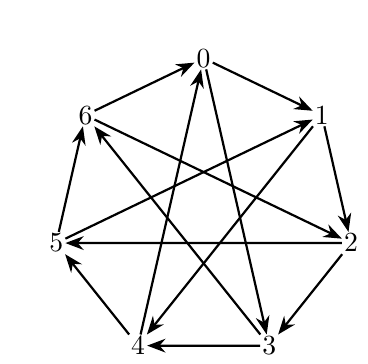
\begin{tikzpicture}[
  scale=0.8,
  >=Stealth,
  node/.style={inner sep=0.6pt}
]
\def\n{7}
\def\r{2.4}

% vertices: 0..6 on a circle (counterclockwise labels)
\foreach \i in {0,...,6} {
  \node[node] (\i) at ({90-360*\i/\n}:\r) {\i};
}

% edges: steps in {1,3}
\foreach \i in {0,...,6} {
  \foreach \s in {1,3} {
    \pgfmathtruncatemacro{\j}{mod(\i+\s,\n)}
    \draw[->,line width=0.8pt] (\i) -- (\j);
  }
}

\end{tikzpicture}
\caption{circulant digraph $\vec{C}_7^{1,3}$}
\label{fig:C713}
\end{figure}


we compute the path homologies of the circulant digraph $\vec{C}_7^{1,3}$ in Example 4.3 of\cite{TY2}: 
\begin{align*}
&H_0^{\mathrm{path}}(\vec{C}_7^{1,3};\K)\cong\K;\\
&H_1^{\mathrm{path}}(\vec{C}_7^{1,3};\K)=\Span_{\K}\bigg\{[e_{03}+e_{36}+e_{60}],[e_{01}+e_{12}+e_{23}+e_{34}+e_{45}+e_{56}+e_{60}]\bigg\};\\
&H_2^{\mathrm{path}}(\vec{C}_7^{1,3};\K)=\Span_{\K}\bigg\{[(e_{014}-e_{034})+(e_{125}-e_{145})+(e_{236}-e_{256})+(e_{340}-e_{360})\\
&\qquad\qquad\qquad\qquad\qquad\quad+(e_{451}-e_{401})+(e_{562}-e_{512})+(e_{603}-e_{623})]\bigg\};\\
&H_m^{\mathrm{path}}(\vec{C}_7^{1,3};\K)=0,\quad m\geq 3.
\end{align*}
But for the symmetric digraph $C_7^{1,3}$, see Fig. \ref{fig:C713pm}. 
\begin{figure}[h]
\centering
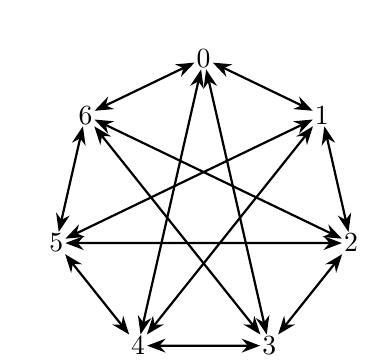
\begin{tikzpicture}[
  scale=0.8,
  >=Stealth,
  node/.style={inner sep=0.6pt}
]
\def\n{7}
\def\r{2.4}

% vertices 0..6 on a circle
\foreach \i in {0,...,6} {
  \node[node] (\i) at ({90-360*\i/\n}:\r) {\i};
}

% edges: step ±1 and ±3  (draw as bidirectional; only need steps 1,3)
\foreach \i in {0,...,6} {
  \pgfmathtruncatemacro{\j}{mod(\i+1,\n)}
  \draw[<->,line width=0.8pt] (\i) -- (\j);

  \pgfmathtruncatemacro{\k}{mod(\i+3,\n)}
  \draw[<->,line width=0.8pt] (\i) -- (\k);
}

\end{tikzpicture}
\caption{circulant graph $C_7^{1,3}$ as a symmetric digraph}
\label{fig:C713pm}
\end{figure}


\noindent Note that the 2-cycle in $\vec{C}_7^{1,3}$ is exactly $W^{1,3}$ in Definition \ref{def:Wcycle}. Now we have
\[S\cup (-S)=\{1,3,-1,-3\}=\{1,3,4,6\}\subset \Z_7.\]
Consider the $3$-paths
\[P^{1,3}=\sum_{a\in\Z_7}e_{a,a+1,a+4,a+5},\qquad P^{4,4}=\sum_{a\in\Z_7}e_{a,a+4,a+1,a+5},\]
by Proposition \ref{prop:P}, we have
\[\partial P^{1,3}=W^{1,4}-W^{1,3},\qquad \partial P^{4,4}=W^{4,1}-W^{4,4}=-W^{1,4}.\]
Then $W^{1,3}$ becomes a boundary
\[W^{1,3}=\partial(-P^{1,3}-P^{4,4}).\]


\end{example}


\begin{remark} The path complex of $C_7^{1,3}$ is still infinite dimensional, and it requires tedious analysis to arrive at its path homology. But it is easy to compute the clique complex\footnote{Clique complex $\mathrm{Cl}(G)$ of a graph $G$ is the simplicial complex whose simplices are cliques (complete subgraphs) of $G$. Thus a 2-simplex exists if and only if $G$ contains a triangle; more generally, $k$-simplices correspond to $(k+1)$-cliques.} of $C_7^{1,3}$ and get the clique homology:
\[H_0(\mathrm{Cl}(C_7^{1,3});\K)\cong\K,\qquad H_1(\mathrm{Cl}(C_7^{1,3});\K)\cong\K,\qquad H_{m\ge 2}(\mathrm{Cl}(C_7^{1,3});\K)\cong0.\]
\end{remark}

\bigskip
\appendix

\section{Two more examples}\label{appendix}

In this appendix, we will analyze the path complexes of $\vec{C}_n^{1,2,4}$ and $\vec{{C}}_n^{1,2,5}$ for $n>10$, and compute the full Betti numbers, i.e. Example \ref{ex:Cn124125}.


\subsection{The circulant digraph \texorpdfstring{$\vec{C}_n^{1,2,4}$, $n>10$}{124}}

First, let us look at the low-dimensional part of its path complex. Using the Fourier bases
\[
v^{(\lambda)}=\sum_a \lambda^{-a}e_a,\qquad
e_s^{(\lambda)}=\sum_a \lambda^{-a}e_{a,a+s},
\]
we have
\[
M_1(t)=\begin{bmatrix} t-1 & t^2-1 & t^4-1\end{bmatrix}.
\]
The Fourier generators of $A_2^{(\lambda)}$ are
\[f_{s_1,s_2}^{(\lambda)}=\sum_a \lambda^{-a}e_{a,a+s_1,a+s_1+s_2}.\]
The space $\Omega_2^{(\lambda)}$ is the subspace of $A_2^{(\lambda)}$ in which illegal middle faces cancel.
Since 
\[1+1=2\in S\quad\text{and}\quad 2+2=4\in S\] 
are the only legal sums, a convenient basis for $\Omega_2^{(\lambda)}$ is
\begin{align*}
\qquad &    A^{(\lambda)}=f_{1,1}^{(\lambda)}, \qquad B^{(\lambda)}=f_{2,2}^{(\lambda)},\\
C^{(\lambda)}=f_{1,2}^{(\lambda)}-f_{2,1}^{(\lambda)},&\qquad D^{(\lambda)}=f_{1,4}^{(\lambda)}-f_{4,1}^{(\lambda)},\qquad E^{(\lambda)}=f_{2,4}^{(\lambda)}-f_{4,2}^{(\lambda)}.
\end{align*}
With respect to the Fourier bases 
\[(e_1^{(\lambda)},e_2^{(\lambda)},e_4^{(\lambda)}) \text{ on } \Omega_1^{(\lambda)} \quad\text{and}
\quad (A^{(\lambda)},B^{(\lambda)},C^{(\lambda)},D^{(\lambda)},E^{(\lambda)}) \text{ on } \Omega_2^{(\lambda)},\]
the symbol matrix $M_2(t)$ for $\partial_2:\Omega_2^{(\lambda)}\to \Omega_1^{(\lambda)}$ is
\[
M_2(t)=
\begin{pmatrix}
t+1 & 0 & 1-t^2 & 1-t^4 & 0\\
-1 & t^2+1 & t-1 & 0 & 1-t^4\\
0 & -1 & 0 & t-1 & t^2-1
\end{pmatrix}.
\]
It's easy to check that $\rank M_2(t)=2$. Then,
\begin{itemize}
    \item for $\lambda\neq1$, we have
    \[\dim H_1^{(\lambda)}=\dim\Omega_1^{(\lambda)}-\rank M_1(\lambda)-\rank M_2(\lambda)=3-1-2=0;\]
    \item for $\lambda=1$, we have
    \[\dim H_1^{(1)}=\dim\Omega_1^{(1)}-\rank M_1(1)-\rank M_2(1)=3-0-2=1.\]
\end{itemize}

In general, we can get a closed-form basis for $\Omega_m$ for all $m\ge 1$.

\smallskip
As before, we write an allowed elementary $m$-path by its step word $w:=(s_1,\dots,s_m)\in \{1,2,4\}^m$ and define the Fourier generator
\[f_w^{(\lambda)}:=f_{s_1,\ldots,s_m}^{(\lambda)}=\sum_{a\in\Z_n}\lambda^{-a}(a;~s_1,\ldots,s_m).\]


For $m\ge 1$, we define the following two kinds of paths:
\begin{itemize}
    \item[(i)] for $0\le k\le m$, define the ``shuffle-alternator''
\[
U_{m,k}:=\sum_{w\in\mathrm{Sh}(1^{m-k},2^k)} (-1)^{\mathrm{inv}(w)}\, f^{(\lambda)}_w,
\]
where $\mathrm{inv}(w)$ counts inversions of the form $(2\text{ before }1)$.
    \item[(ii)] for $0\le k\le m-1$, define the one-$4$ alternator
\[
V_{m,k}:=\sum_{w\in\mathrm{Sh}(1^{m-k-1},2^k,4)} (-1)^{\mathrm{inv}(w)}\, f^{(\lambda)}_w,
\]
with inversion parity computed for the total order $1<2<4$.
\end{itemize}


\begin{lemma}
For $S=\{1,2,4\}$ and every $m\ge 1$,
\[
\Omega_m^{(\lambda)}=\mathrm{Span}\{U_{m,0},\dots,U_{m,m},\, V_{m,0},\dots,V_{m,m-1}\},
\]
hence $\dim \Omega_m^{(\lambda)}= (m+1)+m=2m+1$.
Moreover this basis is independent of $\lambda$.
\end{lemma}

\begin{proof}
For $u\in\Omega_m^{(\lambda)}$, using the Fourier generator $f_w^{(\lambda)}$, we write it as
\[u=\sum_{w\in\{1,2,4\}^m}c_wf_w^{(\lambda)}.\]

\noindent\textbf{Step 1. $\dim \Omega_m^{(\lambda)}\leq 2m+1$:}
Note that the connection set $S=\{1,2,4\}$ satisfies:
\[1+1=2\in S, \quad 2+2=4\in S;\]
while
\[1+2=3\notin S,\quad 1+4=5\notin S, \quad 2+4=6\notin S,\quad 4+4=8\notin S.\]
Fix a position $i\in\{1,\ldots,m-1\}$ and fix the letters of a word outside positions $(i,i+1)$, we have
\begin{itemize}
    \item[(1)] If at positions $(i,i+1)$ the word contains ab with $\{a,b\}\subset\{1,2,4\}$ and $a\neq b$, then
    \[c_{\ldots~ab~\ldots}=-c_{\ldots~ba~\ldots},\quad \text{for } (a,b)\in\{(1,2),(1,4),(2,4)\};\]
    \item[(2)]  If a word contains the adjacent pattern $44$ at some position, then its coefficient is zero:
    \[w \text{ contains } 44~\Rightarrow ~c_w=0.\]
\end{itemize}

Furthermore, for each word $w$, let $w^{\uparrow}$ denote the nondecreasing word obtained by bubble-sorting $w$ using adjacent
swaps. Reuse the above result (1)(2), we understand that every coefficient $c_w$ in $u$ is determined by the coefficient of the sorted word $w^{\uparrow}$ via
\[c_w=(-1)^{\mathrm{inv}(w)}c_{w^{\uparrow}}.\]

For example, 
\begin{itemize}
\setlength{\itemsep}{0pt}
    \item if $w=(2,1,2,1,1)$, then
\[w^{\uparrow}=(1,1,1,2,2),\quad \mathrm{inv}(w)=3+2=5.\]
    \item if $w=(1,4,2,1)$, then
\[w^{\uparrow}=(1,1,2,4),\quad \mathrm{inv}(w)=0+2+1=3.\]
\end{itemize}


Thus, the only sorted words that can carry independent parameters are 
\[1^{m-k}2^k ~~(0\le k\le m),\qquad 1^{m-k-1}2^k4~~(0\le k\le m-1).\]
Thus, $\dim\Omega_m^{(\lambda)}\leq 2m+1$. 

\medskip
\noindent\textbf{Step 2. $U_{m,j}, V_{m,k}\in\Omega_m^{(\lambda)}$ and linearly independent:}
By definition and the above analysis for $u\in\Omega_m^{(\lambda)}$, we know that the illegal faces canceled in $\partial U_{m,j}$ and $\partial V_{m,k}$ respectively. Thus,
\[U_{m,j}, V_{m,k}\in\Omega_m^{(\lambda)}.\]
And it is easy to see that they are linearly independent.
\end{proof}

Next we need to study the symbol matrices $M_m(t)$ for $m\ge 3$ with respect to the ordered basis
\[
\mathcal{B}_m=\bigl(U_{m,0},\dots,U_{m,m},\, V_{m,0},\dots,V_{m,m-1}\bigr).
\]
and compute its rank. Then $M_m(t)$ is the $(2m-1)\times(2m+1)$ matrix representing
$\partial_m:\Omega_m^{(\lambda)}\to\Omega_{m-1}^{(\lambda)}$ under $t=\lambda$.

For completeness, we record explicitly the symbol matrices for $\partial_3$ and $\partial_4$:
\[
M_3(t)=
\begin{pmatrix}
t-1 & t^2-1 & 0 & 0 & 1-t^4 & 0 & 0\\
1 & t+1 & -t^2-1 & 0 & 0 & 1-t^4 & 0\\
0 & 0 & t-1 & t^2-1 & 0 & 0 & 1-t^4\\
0 & 0 & -1 & t+1 & t-1 & t^2-1 & 0\\
0 & 0 & 0 & 0 & 1 & t+1 & t^2-1
\end{pmatrix}.
\]
and
\[
M_4(t)=
\begin{pmatrix}
t+1& 0& 0& 0& 0& 0& 1-t^4& 0& 0\\
-1& t-1& t^2+1& 0& 0& 0& 0& 1-t^4& 0\\
0& 1& t+1& 0& 0& 0& 1& t-1& 0\\
0& 0& -1& t-1& t^2+1& 0& 0& 0& 1-t^4\\
0& 0& 0& 1& t+1& 0& 0& 1& t-1\\
0& 0& 0& 0& -1& t-1& 0& 0& t^2+1\\
0& 0& 0& 0& 0& 1& 0& 0& 1
\end{pmatrix}.
\]
With more efforts, we can see that, for any $n$-th root $\lambda$ (or any $t\in\K$),
\[\rank M_3(\lambda)=3,\qquad \rank M_4(\lambda)=4.\]



\begin{lemma}
For every $m\ge2$, and $n$-th root $\lambda$,
\[\rank M_m(\lambda)=m.\]
\end{lemma}

\begin{proof} We will prove this lemma by the following four steps.

\smallskip
\noindent\textbf{Step 1. Staircase pattern of $M_m(t)$.}
First, for the Fourier generator of the elementary path
\[f_{s_1,\ldots,s_m}^{(\lambda)}=\sum_{a\in\Z_n}\lambda^{-a}e_{a,a+s_1,a+s_1+s_2,\ldots,a+s_1+s_2+\cdots+s_m},\]
we have
\begin{equation}\label{eq:partialf}
\partial f_{s_1,\ldots,s_m}^{(\lambda)}=\lambda^{s_1}f_{s_2,\ldots,s_m}^{(\lambda)}+\sum_{j=1}^{m-1}f_{s_1,\ldots,s_j+s_{j+1},\ldots,s_m}^{(\lambda)}+(-1)^mf_{s_1,\ldots,s_{m-1}}^{(\lambda)}.
\end{equation}
Applying \eqref{eq:partialf} to our $U,V$-type shuffle sums, the only legal merges are $11\rightarrow2$ and $22\rightarrow4$. Then for each $m\ge3$, in terms of the bases $(\mathcal{B}_{m-1},\mathcal{B}_m)$, the matrix
$M_m(t)$ has the following support:
\begin{itemize}
    \item[(i)] The bottom $(m-1)$ rows. Index the bottom rows by $j=0,\ldots,m-2$, corresponding to $V_{m-1,j}$.
Then these rows have a pivot 1 in the $U$-column $U_{m,j+2}$, and the remaining nonzero entries lie in
the $V$–columns near $j$:
\begin{align*}
    \mathrm{Row}~ V_{m-1,2r}:& \quad[\mathrm{Column}~U_{m,2r+2}:1,\quad \mathrm{Column}~V_{m,2r}:t+1,\\
    &~\quad\mathrm{Column}~V_{m,2r+1}:1-t^2;] \\
    \mathrm{Row}~ V_{m-1,2r+1}:& \quad[\mathrm{Column}~U_{m,2r+3}:1,\quad \mathrm{Column}~V_{m,2r}:-1,\\
    &~\quad
    \mathrm{Column}~V_{m,2r+1}:t-1,\quad
    \mathrm{Column}~V_{m,2r+2}:t^2+1.] 
\end{align*}
\item[(ii)] The top $m$ arrows. Index the top rows by $i=0,\ldots,m-1$, corresponding to $U_{m-1,i}$. Then each
row is supported only on three consecutive $U$-columns and one adjacent $V$-column, and the pattern repeats with step 2. 
\end{itemize}


\medskip
\noindent\textbf{Step 2. a universal $(m-1)$-pivot block}

By the statement (i) in Step 1, the bottom $(m-1)$ rows have pivots $1$ in the $U$-columns:
\[U_{m,2},U_{m,3},\ldots,U_{m,m}.\]
These pivots lie in distinct columns, hence the bottom rows are linearly independent and then $\rank M_m(t)\ge m-1$. 


\medskip
\noindent\textbf{Step 3. Lower bound $\rank M_m(t)\ge m$.}
We continue looking at the top row corresponding to $U_{m-1,0}$. By statement (ii), it has a nonzero entry in the column $U_{m,0}$ and is not supported in the pivot columns $U_{m,2},U_{m,3},\ldots,U_{m,m}$. Therefore it cannot be in the span of the bottom rows. Hence $\rank M_m(t)\ge m$.

\medskip
\noindent\textbf{Step 4. Upper bound $\rank M_m(t)\ge m$.}
Using the pivot columns $U_{m,2},\ldots, U_{m,m}$
provided by the bottom rows, perform row operations to eliminate those columns from the top $m$
rows. After this elimination, every remaining top row is supported only on the first two $U$-columns $U_{m,0}, U_{m,1}$ and on the $V$-columns. But the statement (ii) implies that the top block is generated
(after elimination) by at most one independent row (the support repeats in steps of 2, and each
other top row differs from a shift by a combination of the bottom pivot rows). Concretely: for $i\ge 1$
the top row $U_{m-1,i}$ can be reduced to a combination of the bottom row $V_{m-1,i-1}$ (which has pivot
at $U_{m,i+1}$) and neighboring bottom rows, leaving no new pivot in columns $U_{m,0}$ or $U_{m,1}$ beyond the
contribution of $U_{m-1,0}$. Hence the top block contributes at most one additional independent row. Thus, 
$\rank M_m(t)\leq (m-1)+1=m$.
\end{proof}


Using the dimension formula
\[\dim H_m^{(\lambda)}=\dim\Omega_m^{(\lambda)}-\rank M_m(\lambda)-\rank M_{m+1}(\lambda),\]
we arrive at the path homology of $\vec{C}_n^{1,2,4}$ ($n>10$).
\begin{corollary} Let $\lambda$ be the $n$-th root of $1$. 
The path homology of $\vec{C}_n^{1,2,4}$ ($n>10$) is given by
\[H_0^{(\lambda)}\cong\begin{cases}
    \K & \lambda=1\\
    0  & \lambda\neq1
\end{cases},
\qquad 
H_1^{(\lambda)}\cong\begin{cases}
    \K & \lambda=1\\
    0  & \lambda\neq1
\end{cases},
\qquad
H_m^{(\lambda)}\cong0,~~m\ge1.
\]
\end{corollary}

Thus, the Betti numbers are
\[
(\beta_0,\beta_1,\beta_2,\dots)=(1,1,0,\dots),
\]
independent of prime/composite $n$ in the regime $n>10$.

\medskip
\subsection{The circulant digraph \texorpdfstring{$\vec{C}_n^{1,2,5}$, $n>10$}{125}}
Similarly,
\[
M_1(t)=\begin{bmatrix} t-1 & t^2-1 & t^5-1\end{bmatrix}.
\]
Now only $1+1=2$ is a legal sum; a basis for $\Omega_2^{(\lambda)}$ is
\begin{align*}
\qquad &A^{(\lambda)}=f_{1,1}^{(\lambda)}, &&
C_1^{(\lambda)}=f_{1,2}^{(\lambda)}-f_{2,1}^{(\lambda)},\\
\qquad &C_2^{(\lambda)}=f_{1,5}^{(\lambda)}-f_{5,1}^{(\lambda)},&&
C_3^{(\lambda)}=f_{2,5}^{(\lambda)}-f_{5,2}^{(\lambda)}.
\end{align*}

\noindent With respect to $(e_1^{(\lambda)},e_2^{(\lambda)},e_5^{(\lambda)})$ and $(A^{(\lambda)},C_1^{(\lambda)},C_2^{(\lambda)},C_3^{(\lambda)})$,
\[
M_2(t)=
\begin{pmatrix}
t+1 & 1-t^2 & 1-t^5 & 0\\
-1 & t-1 & 0 & 1-t^5\\
0 & 0 & t-1 & t^2-1
\end{pmatrix}.
\]
Similarly, we have
\begin{itemize}
    \item for $\lambda\neq 1$, $\rank{M_2(\lambda)}=2$, then
    \[\dim H_1^{(\lambda)}=\dim\Omega_1^{(\lambda)}-\rank M_1(\lambda)-\rank M_2(\lambda)=3-1-2=0;\]
    \item for $\lambda=1$, $\rank{M_2(1)}=1$, then
    \[\dim H_1^{(1)}=\dim\Omega_1^{(1)}-\rank M_1(1)-\rank M_2(1)=3-0-1=2.\]
\end{itemize}





In general, define four generators for each $m\ge 2$:
\begin{align*}
\qquad &A_m := f^{(\lambda)}_{1,1,\dots,1}, &&
B_m := \sum_{i=0}^{m-1} (-1)^{m-1-i}f^{(\lambda)}_{1^i,2,1^{m-1-i}},\\
\qquad &C_m := \sum_{i=0}^{m-1} (-1)^{m-1-i} f^{(\lambda)}_{1^i,5,1^{m-1-i}}, && D_m := \sum_{w\in \mathrm{Sh}(1^{m-2},2,5)} (-1)^{\mathrm{inv}(w)} f^{(\lambda)}_{w},
\end{align*}
where inversion parity uses $1<2<5$.

\vskip 0.1cm
Continue the discussion as we have done for $\vec{C}_n^{1,2,4}$, we have
\begin{lemma}
For $S=\{1,2,5\}$ and every $m\ge 2$, $\Omega_m$ is 4 dimensional, and
\[
\Omega_m^{(\lambda)}=\mathrm{Span}\{A_m,B_m,C_m,D_m\}.
\]
\end{lemma}

Using the ordered basis $\mathcal{C}_m=(A_m,B_m,C_m,D_m)$, the differential
$\partial_m$ is represented by one of two matrices depending on the parity of $m$:

\medskip\noindent
\textbf{Odd $m$ (e.g.\ $m=3,5,\dots$):}
\[
M_m(t)=
\begin{pmatrix}
t-1 & t^2-1 & t^5-1 & 0\\
1 & t+1 & 0 & 1-t^5\\
0 & 0 & t+1 & t^2-1\\
0 & 0 & 1 & t-1
\end{pmatrix}.
\]

\medskip\noindent
\textbf{Even $m$ (e.g.\ $m=4,6,\dots$):}
\[
M_m(t)=
\begin{pmatrix}
t+1 & 1-t^2 & 1-t^5 & 0\\
-1 & t-1 & 0 & 1-t^5\\
0 & 0 & t-1 & t^2-1\\
0 & 0 & 1 & t+1
\end{pmatrix}.
\]

Computing ranks on each Fourier block gives 
\[\rank M_m(\lambda)=2,\quad \forall m\ge 3,~\lambda^n=1.\]
Furthermore, it gives the Betti numbers:
\[
\beta_0=1,\quad \beta_1=2,\quad \beta_2=1,\quad \beta_m=0\ (m\ge 3).
\]
This completes the computation for all higher degrees. Again the result is independent of prime/composite $n$ when $n>10$.



\bigskip

\begin{thebibliography}{0}

\bibitem{ABTW} A. Ahmadi, R. Belk, C. Tamon, and C. Wendler,
\textit{On mixing in continuous-time quantum walks on some circulant graphs}.
\text{Quantum Information \& Computation}, Volume 3, Issue 6 (2003), 611--618.

\bibitem{Alspach2002}
B.~Alspach and T.~Dixon,
\textit{Enumeration of Cayley graphs and digraphs}.
J.\ Combin.\ Theory Ser.\ B 86 (2002), 50--62.




\bibitem{BCH95}
J.-C.~Bermond, F.~Comellas, and D.~F.~Hsu,
\textit{Distributed loop computer networks: a survey}. 
Journal of Parallel and Distributed Computing
\textbf{24}(1) (1995), 2--10.


\bibitem{Biggs} N. Biggs, 
\textit{Algebraic Graph Theory, 2nd ed}. 
Cambridge Mathematical Library (Cambridge University Press, Cambridge, 1993).

\bibitem{BoeschTindell84}
F.~Boesch and R.~Tindell,
\textit{Circulants and their connectivities}.
Journal of Graph Theory \textbf{8}(4) (1984), 487--499.
DOI: 10.1002/jgt.3190080406.


\bibitem{ChowdhuryMemoli2017}
S.~Chowdhury and F.~M\'emoli,
\textit{Persistent path homology of directed networks}.
arXiv:1701.00565 (2017).

\bibitem{CirculantThesis2016}
E.~Cancela,
\textit{Circulant Digraph Isomorphisms}.
Ph.D. thesis, Mississippi State University (2016).


\bibitem{Davis1979}
P.~J.~Davis,
\textit{Circulant Matrices}.
Wiley--Interscience, New York, 1979.



\bibitem{DIMZ} S. Di, S. O. Ivanov, L. Mukoseev, and M. Zhang,
\textit{On the path homology of Cayley digraphs and covering digraphs}.
Journal of Algebra, Vol 653 (2024), 156--199.

\bibitem{Fossorier04}
M.~P.~C.~Fossorier,
\textit{Quasi-cyclic low-density parity-check codes from circulant permutation matrices}.
IEEE Transactions on Information Theory, \textbf{50}(8) (2004), 1788--1793.


\bibitem{FI} X. Fu, and S. O. Ivanov,
\textit{Path homology of digraphs without multisquares and its comparison with homology of spaces}.
arXiv:2407.17001.


\bibitem{Gray2006} R.~M.~Gray,
\textit{Toeplitz and Circulant Matrices: A Review}.
Foundations and Trends in Communications and Information Theory
\textbf{2}(3) (2006), 155--239.
%DOI: 10.1561/0100000006.

\bibitem{Grigoryan} A. Grigoryan,
\textit{dslides, a series talk of (co)holomology theory of digraph}.
\href{dslides}{https://www.math.uni-bielefeld.de/~grigor/dslides.pdf}


\bibitem{GrigoryanHodge} A. Grigoryan,
\textit{Path homology and Hodge Laplacian on digraphs}.
\href{dslides}{https://www.math.uni-bielefeld.de/~grigor/hodge2.pdf}



\bibitem{GLMY:basic} A. Grigoryan, Y. Lin, Y. Muranov, and S.-T. Yau,
\textit{Homologies of Path Complexes and Digraphs}.
preprint, 2012. http://arxiv.org/abs/1207.2834


\bibitem{GLMY:homotopy} A. Grigoryan, Y. Lin, Y. Muranov, and S.-T. Yau,
\textit{Homotopy Theory for Digraphs}.
Pure and Applied Math. Quarterly 10 (2014), 619-674.

\bibitem{GLMY:cohomology} A. Grigoryan, Y. Lin, Y. Muranov, and S.-T. Yau,
\textit{Cohomology of Digraphs and (Undirected) Graphs}.
Asian J. Math. 19 (2015), 887-932.


\bibitem{GLYZ:eigenvalues} A. Grigoryan, Y. Lin, S.-T. Yau, and H. Zhang,
\textit{Eigenvalues of the Hodge Laplacian on digraphs}.
Comm. Anal. Geom. 33 (2025), No. 4, 981-1023.



\bibitem{GMY:product} A. Grigoryan, Y. Muranov, and S.-T. Yau,
\textit{Homologies of Digraphs and K\"unneth Formulas}.
Comm. Anal. Geom. 25 (2017), 969-1018.


\bibitem{HRD2022} X. Huang, A. F. Ramos, and Y. Deng,
\textit{Optimal circulant graphs as low-latency network topologies}.
The Journal of Supercomputing, Volume 78 (2022), 13491--13510.


\bibitem{Hwang03}
F.~K.~Hwang,
\textit{A survey on multi-loop networks}.
Theoretical Computer Science \textbf{299} (2003), 107--121.


\bibitem{IP} S. O. Ivanov, and F. Pavutnitskiy,
\textit{Simplicial Approach to Path Homology of Quivers, Marked Categories, Groups and Algebras}.
Journal of the London Mathematical Society, 2024, 109(1): e12812.




\bibitem{LMWY} J. Li, Y. Muranov, J. Wu, and S.-T. Yau, 
\textit{On singular homology theories of digraphs and quivers}. accepted by Journal of Combinatorics (2025).


\bibitem{LWY} Y. Lin, C. Wang and S.-T. Yau,
\textit{Discrete Morse Theory on Digraphs}.
Pure and Applied Math. Quarterly 17(5) (2021), 1711--1737.


\bibitem{Louis} 
J.~Louis,
\textit{Asymptotics for the number of spanning trees in circulant graphs and deconnection $d$-dimensional discrete tori}.
Ann. Comb. (2015), 1-31.


\bibitem{MBGcoding} C. Martinez, R. Beivide, and E. Gabidulin,
\textit{Perfect Codes for Metrics Induced by Circulant Graphs}.
in IEEE Transactions on Information Theory, vol. 53 (2007), no. 9, 3042--3052.

\bibitem{Morris06Survey}
J.~Morris,
\textit{Automorphism Groups of Circulant Graphs --- a Survey}.
in: A.~Bondy, J.~Fonlupt, J.-L.~Fouquet, J.-C.~Fournier, J.-L.~Ram\'{\i}rez Alfons\'{\i}n (eds.),
\textit{Graph Theory in Paris},
Trends in Mathematics, Birkh\"auser Basel, (2006), 311--325. arXiv:math/0411302.

\bibitem{TY1} X. Tang, and S.-T. Yau,
\textit{Minimal Path and Acyclic Model in the Path Complex}.
Comm. Ana. Geom. 33 (2), 275-342; arXiv:2208.14063v2.


\bibitem{TY2} X. Tang, and S.-T. Yau,
\textit{The Cellular Homology of Digraphs}.
arXiv:2402.05682v2. Accepted by Asian J. Math.



\bibitem{CayleyMathWorld}
E.~W.~Weisstein,
\textit{Cayley Graph}. MathWorld--A Wolfram Web Resource.%\newline
%\href{https://mathworld.wolfram.com/CayleyGraph.html}{https://mathworld.wolfram.com/CayleyGraph.html}


\end{thebibliography}



\end{document}